
% chapters/tikz_ch08.tex - 第 8 章插图 (TikZ 全矢量重绘)
% 图 8.1 光锥与零双特征线; 图 8.2 实主型传播估计

% ============ 图 8.1 ============
\newcommand{\drawFigEightOne}{%
\begin{tikzpicture}[scale=1.0, >=stealth, line join=round]
    % ---------- 左图: 波动算子的特征集 ----------
    \begin{scope}[shift={(0,0)}]
        \draw[->] (0.25,0.25) -- (5.9,0.25) node[right, font=\small] {$x$};
        \draw[->] (0.25,0.25) -- (0.25,5.20) node[above, font=\small] {$t$};
        % 双光锥 1
        \coordinate (P0) at (1.40,1.00);
        \draw[thick] (P0) -- ++(0.85,0.85);
        \draw[thick] (P0) -- ++(-0.85,0.85);
        \draw[thick] (P0) -- ++(0.60,-0.60);
        \draw[thick] (P0) -- ++(-0.60,-0.60);
        \fill (P0) circle (1.6pt);
        \node[below left, font=\small] at (1.42,0.96) {$(t_0,x_0)$};
        % 双光锥 2
        \coordinate (P1) at (4.40,4.00);
        \draw[thick] (P1) -- ++(0.85,0.85);
        \draw[thick] (P1) -- ++(-0.85,0.85);
        \draw[thick] (P1) -- ++(0.60,-0.60);
        \draw[thick] (P1) -- ++(-0.60,-0.60);
        \fill (P1) circle (1.6pt);
        \node[right, font=\small] at (4.46,4.02) {$(t_1,x_1)$};
        % 零双特征线上的两个点与底投影
        \coordinate (A) at (1.95,1.55);
        \coordinate (B) at (3.85,3.45);
        \fill[gray!70] (A) circle (2.2pt);
        \fill[gray!70] (B) circle (2.2pt);
        \draw[very thick, gray!70] (A) -- (B);
        \draw[densely dashed, gray] (A) -- ($(A)-(0,0.55)$);
        \draw[densely dashed, gray] (B) -- ($(B)-(0,0.55)$);
    \end{scope}
    % ---------- 右图: 乘子算子的零双特征线 ----------
    \begin{scope}[shift={(6.55,0.55)}]
        \draw[->] (0,0) -- (4.70,0) node[right, font=\small] {$\xi$};
        \node[below left, font=\small] at (0.02,-0.02) {$0$};
        \fill (1.30,0) circle (1.6pt);
        \node[below, font=\small] at (1.30,-0.06) {$\xi_0$};
        \fill[gray!70] (3.30,0) circle (2.2pt);
        \node[below, font=\small] at (3.30,-0.06) {$\xi_0+s\tilde{\xi}$};
        \draw[very thick, gray!70, ->] (1.42,0) -- (3.18,0);
        \node[above, font=\small] at (2.35,0.55) {$-\partial_x p_4(x_0)$};
        \draw[->] (2.35,0.45) -- (2.95,0.08);
        \node[above, font=\small] at (1.30,0.95) {纤维 $T^*_{x_0}\R^n$};
        \node[font=\small] at (2.35,-1.15) {$\operatorname{Char}(P_4)=\{p_4(x_0)=0,\ \xi\neq 0\}$};
    \end{scope}
\end{tikzpicture}}

% ============ 图 8.2 ============
\newcommand{\drawFigEightTwo}{%
\begin{tikzpicture}[scale=1.0, >=stealth]
    % 邻域 U
    \draw[gray, densely dashed, rounded corners=8pt] (0.20,0.35) rectangle (8.20,3.55);
    \node[gray, font=\small, anchor=north east] at (8.10,3.48) {$\mathcal{U}$};
    % 零双特征线
    \draw[very thick] (1.30,1.00) .. controls (3.20,1.05) and (5.40,2.65) .. (7.30,3.00);
    \fill (1.30,1.00) circle (1.8pt);
    \node[below left, font=\small] at (1.30,0.92) {$\gamma(0)$};
    \fill (7.30,3.00) circle (1.8pt);
    \node[above right, font=\small] at (7.32,3.06) {$\gamma(s_0)$};
    % Ell(E)
    \draw[very thick, gray!60, fill=gray!12] (1.30,1.00) ellipse (0.95 and 0.62);
    \node[font=\small] at (1.30,1.82) {$\Ell(E)$};
    % Ell(B): 沿曲线的灰带
    \draw[line width=9pt, gray!25, line cap=round] (2.35,1.02) .. controls (3.40,1.25) and (5.20,2.55) .. (6.55,2.93);
    \node[font=\small] at (4.55,1.35) {$\Ell(B)$};
    % 右侧说明
    \node[font=\small, anchor=west, align=left] at (0.40,3.15)
        {在此 $\gamma$ 的邻域内 $GPu\in H^{s-m+1}$};
    \draw[->, gray] (2.55,3.02) -- (4.10,2.72);
\end{tikzpicture}}

% ============ 图 8.3 ============
\newcommand{\drawFigEightThree}{%
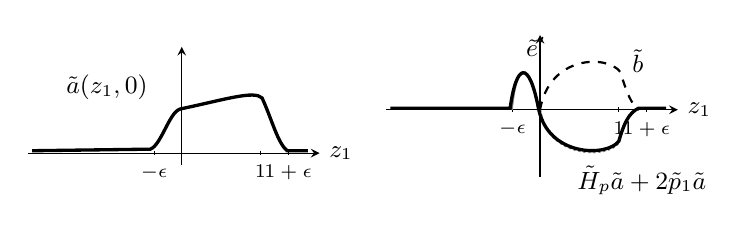
\begin{tikzpicture}[scale=1.0, >=stealth]
    % ---------- 左图: 对易子 \tilde a 的图像 ----------
    \begin{scope}[shift={(0,0)}]
        \draw[->] (-1.95,0) -- (1.75,0) node[right, font=\small] {$z_1$};
        \draw[->] (0,-0.15) -- (0,1.35);
        \foreach \x/\lab in {-0.35/{-\epsilon}, 1.0/{1}, 1.35/{1+\epsilon}}
            \draw (\x,0.03) -- (\x,-0.03) node[below, font=\scriptsize] {$\lab$};
        \draw[very thick] (-1.90,0.03) -- (-0.40,0.05)
            .. controls (-0.26,0.10) and (-0.16,0.52) .. (-0.02,0.56)
            .. controls (0.55,0.68) and (0.92,0.80) .. (1.02,0.70)
            .. controls (1.14,0.44) and (1.22,0.12) .. (1.34,0.03)
            -- (1.60,0.03);
        \node[above, font=\small] at (-0.95,0.55) {$\tilde{a}(z_1,0)$};
    \end{scope}
    % ---------- 右图: (8.46) 中的各项 ----------
    \begin{scope}[shift={(4.55,0.55)}]
        \draw[->] (-1.95,0) -- (1.75,0) node[right, font=\small] {$z_1$};
        \draw[->] (0,-0.85) -- (0,0.95);
        \foreach \x/\lab in {-0.35/{-\epsilon}, 1.0/{1}, 1.35/{1+\epsilon}}
            \draw (\x,0.03) -- (\x,-0.03) node[below, font=\scriptsize] {$\lab$};
        % \tilde e' 的正尖峰
        \draw[thick, gray] (-0.36,0) .. controls (-0.30,0.62) and (-0.14,0.66) .. (-0.02,0);
        % -\tilde b^2 的负平台
        \draw[thick, gray, densely dotted] (0,0) .. controls (0.10,-0.62) and (0.85,-0.62) .. (1.00,-0.42)
            .. controls (1.06,-0.18) and (1.12,-0.05) .. (1.22,0);
        % 合成曲线 H_p a + 2 p_1 a
        \draw[very thick] (-1.90,0.02) -- (-0.38,0.02)
            .. controls (-0.30,0.60) and (-0.14,0.64) .. (-0.02,0.02)
            .. controls (0.10,-0.60) and (0.85,-0.60) .. (1.00,-0.40)
            .. controls (1.07,-0.16) and (1.13,-0.04) .. (1.25,0.02)
            -- (1.60,0.02);
        % \tilde b
        \draw[thick, dashed] (0,0) .. controls (0.12,0.70) and (0.86,0.70) .. (1.02,0.48)
            .. controls (1.10,0.22) and (1.16,0.06) .. (1.26,0);
        \node[font=\small, anchor=west] at (0.35,-0.90) {$\tilde{H}_p\tilde{a}+2\tilde{p}_1\tilde{a}$};
        \node[font=\small, anchor=west] at (1.05,0.62) {$\tilde{b}$};
        \node[font=\small, anchor=west] at (-0.30,0.80) {$\tilde{e}'$};
    \end{scope}
\end{tikzpicture}}

% ============ 图 8.4 ============
\newcommand{\drawFigEightFour}{%
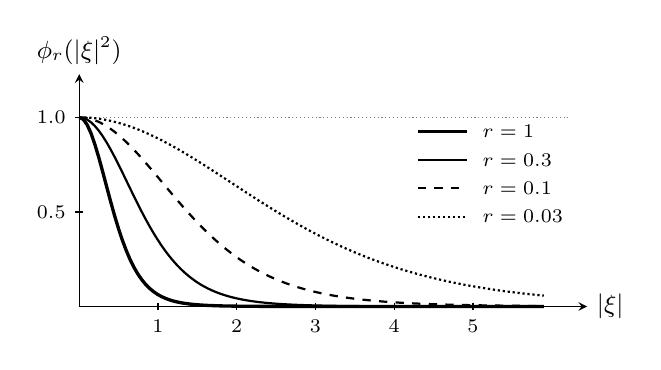
\begin{tikzpicture}[scale=1.0, >=stealth]
    \draw[->] (0,0) -- (6.45,0) node[right, font=\small] {$| \xi |$};
    \draw[->] (0,0) -- (0,2.95) node[above, font=\small] {$\phi_r(| \xi |^2)$};
    \foreach \x in {1,2,3,4,5} \draw (\x,0.05) -- (\x,-0.05) node[below, font=\scriptsize] {$\x$};
    \foreach \y/\lab in {1.20/{0.5}, 2.40/{1.0}}
        \draw (0.05,\y) -- (-0.05,\y) node[left, font=\scriptsize] {$\lab$};
    \draw[gray, densely dotted] (0,2.40) -- (6.20,2.40);
    % r = 1, 0.3, 0.1, 0.03
    \draw[very thick] plot[domain=0:5.9, samples=120] (\x, {2.4*(1+1.0*\x*\x)^(-4)});
    \draw[thick] plot[domain=0:5.9, samples=120] (\x, {2.4*(1+0.3*\x*\x)^(-4)});
    \draw[thick, dashed] plot[domain=0:5.9, samples=120] (\x, {2.4*(1+0.1*\x*\x)^(-4)});
    \draw[thick, densely dotted] plot[domain=0:5.9, samples=120] (\x, {2.4*(1+0.03*\x*\x)^(-4)});
    % 图例 (置于曲线均已衰减的空白区)
    \draw[very thick] (4.30,2.22) -- (4.92,2.22);
    \node[font=\scriptsize, anchor=west] at (5.00,2.22) {$r = 1$};
    \draw[thick] (4.30,1.86) -- (4.92,1.86);
    \node[font=\scriptsize, anchor=west] at (5.00,1.86) {$r = 0.3$};
    \draw[thick, dashed] (4.30,1.50) -- (4.92,1.50);
    \node[font=\scriptsize, anchor=west] at (5.00,1.50) {$r = 0.1$};
    \draw[thick, densely dotted] (4.30,1.14) -- (4.92,1.14);
    \node[font=\scriptsize, anchor=west] at (5.00,1.14) {$r = 0.03$};
\end{tikzpicture}}

% ============ 图 8.5 ============
\newcommand{\drawFigEightFive}{%
\begin{tikzpicture}[scale=1.0, >=stealth]
    % S^*M 边框
    \draw[gray, densely dashed, rounded corners=6pt] (0.30,0.30) rectangle (9.10,4.20);
    \node[gray, font=\small, anchor=north east] at (9.00,4.12) {$S^*M$};
    % Char(P) 曲线
    \draw[thick] (0.70,1.55) .. controls (3.00,1.20) and (5.60,2.90) .. (8.60,2.55);
    \node[font=\small, anchor=west] at (8.62,2.55) {$\operatorname{Char}(P)$};
    % Ell(G)：沿曲线的灰带
    \draw[line width=13pt, gray!22, line cap=round] (0.95,1.52) .. controls (3.05,1.22) and (5.60,2.86) .. (8.05,2.60);
    \node[font=\small] at (4.35,1.02) {$\Ell(G)$};
    % Ell(E)：左端圆盘
    \draw[very thick, gray!60, fill=gray!15] (1.35,1.46) ellipse (0.72 and 0.52);
    \node[font=\small] at (1.35,2.28) {$\Ell(E)$};
    % WF'(B) ∩ Char(P)：右端阴影块
    \fill[gray!45, rounded corners=4pt] (6.70,2.30) rectangle (8.30,2.92);
    \node[font=\small, anchor=south] at (7.50,2.96) {$\WF'(B)\cap\operatorname{Char}(P)$};
    % 后向零双特征线（箭头指向 Ell(E)）
    \draw[->, thick, gray!70] (6.75,2.55) .. controls (5.20,2.72) and (3.10,1.80) .. (2.05,1.55);
    \draw[->, thick, gray!70] (6.90,2.85) .. controls (5.00,3.10) and (2.90,2.20) .. (2.00,1.85);
    \node[font=\small, anchor=west] at (3.85,3.55) {后向零双特征线};
    \draw[->, gray] (3.80,3.42) -- (3.05,2.72);
\end{tikzpicture}}

% ============ 图 8.6 ============
% 例 8.22: P = hD_x - a 的特征集与 H_p 的流
\newcommand{\drawFigEightSix}{%
\begin{tikzpicture}[scale=1.0, >=stealth, line join=round]
    % 坐标轴
    \draw[->] (0.10,2.10) -- (7.55,2.10) node[below right, font=\small] {$x$};
    \draw[->] (4.00,0.15) -- (4.00,4.35) node[above, font=\small] {$\xi$};
    % 特征集 Char_h(P) = { xi = a(x) }, 同时也是 H_p 的一条积分曲线
    \draw[line width=1.1pt,
          postaction={decorate, decoration={markings,
            mark=at position 0.135 with {\arrow{stealth}},
            mark=at position 0.435 with {\arrow{stealth}},
            mark=at position 0.705 with {\arrow{stealth}},
            mark=at position 0.915 with {\arrow{stealth}}}}]
        (0.35,4.02)
        .. controls (1.00,4.18) and (1.50,3.98) .. (2.02,3.60)
        .. controls (2.42,3.34) and (2.68,3.30) .. (2.95,3.22)
        .. controls (3.35,3.10) and (3.62,2.60) .. (3.96,2.10)
        .. controls (4.36,1.52) and (4.86,0.94) .. (5.55,0.80)
        .. controls (6.10,0.70) and (6.58,1.06) .. (7.05,1.46);
    % 标注
    \node[font=\small, anchor=east] (charP) at (1.95,4.62) {$\Char_\hbar(P)$};
    \draw[->, gray] (charP.east) -- (1.28,4.10);
    \node[font=\small, anchor=north] (Hp) at (5.72,0.62) {$H_p$};
    \draw[->, gray] (Hp.north) -- (5.62,0.76);
\end{tikzpicture}}


\chapter[实主型奇性传播]{实主型奇性传播}\label{ch:08}
\index{shi zhuxing@实主型 (real principal type)}%
\index{zheng duiyizi@正对易子 (positive commutator)}%

我们现在摆脱前章那种方程明显以演化形式给出的限制性框架. 在第~\ref{sec:8.1}~至~\ref{sec:8.6}~节中, 我们证明一般非椭圆 (伪) 微分方程
\begin{equation}\label{eq:8.1}
    Pu = f, \qquad P \in \Psi^m(M)
\end{equation}
的解的奇性 (波前集) 的传播, 等价地, 正则性的传播, 其中 $M = \R^n$ 或别的流形, $m \in \R$. 我们假定主符号
\begin{equation}\label{eq:8.2}
    p(x, \xi) \defeq \sigma^m(P)(x, \xi) \in S^m_{\mathrm{hom}}(T^*M \setminus o)
\end{equation}
是 $m$ 次齐次的 (当 $P$ 是微分算子时这自动成立) 且取实值. (所谓属于~\eqref{eq:8.2}, 我们指 $(1 - \chi)p$ 是 $\sigma^m(P) \in S^m(T^*M)/S^{m-1}(T^*M)$ 的一个代表元, 其中 $\chi \in \Smooth(T^*M)$ 在零截面附近等于 $1$, 在纤维无穷远附近等于 $0$.) 半经典情形在第~\ref{sec:8.7}~节处理.

\section{定理的陈述; 第一个证明}\label{sec:8.1}

我们首先给出一些算子的例子, 供读者在本章中随时对照. 前两个例子是演化形式的. 即便对它们, 我们这里证明的奇性传播结果也与定理~\ref{thm:7.8} 有定性上的不同, 因为我们现在追踪的是 $u$ 在 $M$ 上的波前集, 而非 $u$ 限制到时间函数的水平集上的波前集.

\begin{example}[具有实主符号的算子]\label{eg:8.1}
\begin{enumerate}
    \item (输运算子.) 在 $M = \R_t \times \R^{n-1}_x$ 上, 对实值函数 $a_j \in \Smooth(M)$, $j = 1, \ldots, n-1$, 算子
    \begin{equation}\label{eq:8.3}
        P_1 \defeq D_t, \qquad P_2 \defeq D_t + \sum_{j=1}^{n-1} a_j(t, x) D_{x_j} \in \operatorname{Diff}^1(M)
    \end{equation}
    具有实主符号. 把余向量写作 $\tau \dd t + \sum_{j=1}^{n-1} \xi_j \dd x_j$, 它们就是
    \begin{equation}\label{eq:8.4}
        p_1(t, x, \tau, \xi) = \tau, \qquad p_2(t, x, \tau, \xi) = \tau + \sum_{j=1}^{n-1} a_j(t, x)\xi_j.
    \end{equation}
    \item (波动算子.) 另一个具有实主符号的微分算子是波动算子
    \begin{equation}\label{eq:8.5}
        P_3 \defeq -D_t^2 + \sum_{j=1}^{n-1} D_{x_j}^2 \in \operatorname{Diff}^2(M), \qquad p_3(t, x, \tau, \xi) = -\tau^2 + | \xi |^2.
    \end{equation}
    \item (乘子算子.) 在任意光滑流形 $M$ 上, 取 $p_4 \in \Smooth(M; \R)$, 并考虑算子 $P_4 \colon u \mapsto p_4 u$. 则 $P_4 \in \Psi^0(M)$ 具有实主符号 $p_4$.
\end{enumerate}
\end{example}

\begin{definition}[零双特征线]\label{def:8.2}
$P$ 的一条 (\textbf{前向}) \textbf{零双特征线} (null-bicharacteristic) 是 Hamilton 向量场 $H_p$ 的一条位于 $\operatorname{Char}(P) \subset T^*M \setminus o$ 中的积分曲线. 我们对 $\operatorname{Char}(P) \subset S^*M$ 中那些作为 $S^*M = (T^*M \setminus o)/\R_+$ 中零双特征线之像的光滑曲线 (或它们的光滑单调重参数化) 也使用同一术语. $P$ 的\textbf{后向}零双特征线是 $-P$ 的前向零双特征线.
\end{definition}

注意 $H_p p = 0$; 因此, $H_p$ 的以 $\alpha \in \operatorname{Char}(P)$ 为初值的积分曲线自动是零双特征线, 且所有零双特征线都由此方式得到.

\begin{example}[零双特征线]\label{eg:8.3}
我们考察例~\ref{eg:8.1} 中的算子.
\begin{enumerate}
    \item (输运算子.) 由于 $\operatorname{Char}(P_1) = \{(t, x, \tau, \xi) \colon \tau = 0, \; \xi \neq 0\}$ 且 $H_{p_1} = \partial_t$, $P_1$ 的零双特征线是曲线 $s \mapsto (t_0 + s, x_0; 0, \xi_0)$. 对~\eqref{eq:8.3} 中更一般的算子 $P_2$, 我们有
    \begin{equation}\label{eq:8.6}
        H_{p_2} = \left( \partial_t + \sum_{j=1}^{n-1} a_j(t, x)\partial_{x_j} \right) - \sum_{j=1}^{n-1} \xi_j \left( \partial_t a_j(t, x)\partial_\tau + \sum_{k=1}^{n-1} \partial_{x_k} a_j(t, x)\partial_{\xi_k} \right).
    \end{equation}
    于是零双特征线 (事实上 $H_{p_2}$ 的所有积分曲线) 投影到 $M$ 上恰好就是输运向量场 $\partial_t + \sum_{j=1}^{n-1} a_j(t, x)\partial_{x_j}$ 的积分曲线.
    \item (波动算子.) 我们有 $\operatorname{Char}(P_3) = \{(t, x, \tau, \xi) \colon | \xi | = | \tau | \neq 0\}$. 于是 $\operatorname{Char}(P_3) \cap (T^*_{(t_0, x_0)}M \setminus o)$ 是一个双锥 (去掉顶点), 称为 (\textbf{对偶}) \textbf{光锥}. 我们有
    \begin{equation}\label{eq:8.7}
        H_{p_3} = -2\tau \partial_t + 2\xi \cdot \partial_x,
    \end{equation}
    其中 $\xi \cdot \partial_x \defeq \sum_{j=1}^{n-1} \xi_j \partial_{x_j}$. 注意 $H_p \tau = 0$, 故 $\tau$ 沿零双特征线为常数. 沿其 $\tau = -1$ 的零双特征线由
    \begin{equation}\label{eq:8.8}
        s \mapsto (t_0 + 2s, x_0 + 2\xi_0 s; -1, \xi_0), \qquad | \xi_0 | = 1
    \end{equation}
    给出. 它们到 $M$ 的投影是零测地线. 见图~\ref{fig:8.1} 左图.
    \item (乘子算子.) 在 $M$ 的局部坐标 $x \in \R^n$ 中, 我们有 $\operatorname{Char}(P_4) = \{(x, \xi) \colon p_4(x) = 0, \; \xi \neq 0\}$, 且
    \begin{equation}\label{eq:8.9}
        H_{p_4} = -(\partial_x p_4) \cdot \partial_\xi.
    \end{equation}
    于是在满足 $p_4(x_0) = 0$ 的点 $x_0 \in \R^n$ 处, 零双特征线停留在纤维 $T^*_{x_0}\R^n \setminus o$ 中, 但在动量变量中沿方向 $-\partial_x p_4(x_0)$ 运动. 见图~\ref{fig:8.1} 右图.
\end{enumerate}
\end{example}

本章主要结果的第一种表述如下.

\begin{theorem}[奇性传播: 光滑情形]\label{thm:8.4}
设 $P \in \Psi^m(M)$ (适正支集) 具有实值齐次主符号. 设 $u \in \Distr(M)$, 并假定 $Pu \in \Smooth(M)$. 则 $\WF(u) \subset \operatorname{Char}(P)$ 是 $P$ 的极大延拓零双特征线之并.
\end{theorem}

$\WF(u) \subset \operatorname{Char}(P)$ 这一断言由微局部椭圆正则性 (命题~\ref{prop:6.33}) 得到. 该定理断言: 在 $\operatorname{Char}(P)$ 内, ``微局部解'' $u$ (即满足 $\WF(Pu) = \emptyset$ 者) 的波前集在 $H_p$-流下不变. 与其把定理~\ref{thm:8.4} 称为奇性传播的结果, 人们常常 (也更有用地) 把它视为\textbf{正则性传播}的结果, 因为 $\alpha \notin \WF(u) \cap \operatorname{Char}(P)$ 蕴含过 $\alpha$ 的 $P$ 的极大延拓零双特征线与 $\WF(u)$ 不相交.

\begin{figure}[htbp]
\centering
\drawFigEightOne
\caption{左图: 我们图示波动算子 $P_3$ 在两个点 $(t_0, x_0)$, $(t_1, x_1)$ 上的特征集 (即对偶光锥), 并在其上标出位于同一条 $P_3$ 的零双特征线上的两个点. 实线是该零双特征线的底投影. 右图: $P_4$ 的零双特征线的类似图示.}
\label{fig:8.1}
\end{figure}

\begin{proof}[定理~\ref{thm:8.4} 的证明]
我们把它化归为局部结果. 若 $\chi, \tilde{\chi} \in \SmoothComp(M)$ 是两个切断函数, 且 $\tilde{\chi} \equiv 1$ 于 $\operatorname{supp}\chi$ 附近, 则
\begin{equation}\label{eq:8.10}
    \chi P \tilde{\chi} u = \chi P u + \chi [P, \tilde{\chi}] u \in \SmoothComp(M).
\end{equation}
我们在此用到 $\chi [P, \tilde{\chi}] \in \Psi^{-\infty}(M)$. 于是, 若 $\phi \in \SmoothComp(M)$ 在 $\operatorname{supp}\tilde{\chi}$ 附近恒等于 $1$, 我们可以用 $\chi P \tilde{\chi}$ 代替 $P$, 用 $\phi u$ 代替 $u$, 而仍保持 $Pu \in \Smooth(M)$; 此外, 这些替换不改变 $P$ 的零双特征线, 也不改变 $\chi^{-1}(1)$ 上方相空间中 $u$ 的波前集. 如此局部化到坐标卡之后, 我们可以假定
\begin{equation}\label{eq:8.11}
    P \in \Psi^m(\R^n), \quad u \in \mathcal{E}'(\R^n), \quad Pu = f \in \SmoothComp(\R^n).
\end{equation}
我们用 $\Lambda \defeq \langle D \rangle^{m-1}$ 作规范化: 把 $(P, u)$ 换成 $(P\Lambda^{-1}, \Lambda u)$, 并再次应用上述局部化论证; 于是可以假定 $m = 1$. 经这些替换后, $P$ 的主符号仍然是齐次且实值的.

现在我们引入一个人为的时间变量 $t$, 并令
\begin{equation}\label{eq:8.12}
    \tilde{u}(t, x) \defeq u(x), \qquad \tilde{f}(t, x) \defeq f(x).
\end{equation}
则 $\tilde{u}$ 解方程
\begin{equation}\label{eq:8.13}
    (D_t + P)\tilde{u} = \tilde{f}.
\end{equation}
定理~\ref{thm:7.8} 与注~\ref{rem:7.9} 蕴含
\begin{equation}\label{eq:8.14}
    \WF(u) = \WF(\tilde{u}(t)) = \mathcal{C}(t, 0)\WF(\tilde{u}(0)) = \mathcal{C}(t, 0)\WF(u),
\end{equation}
其中 $\mathcal{C}(t, 0)$ 是 $H_p$ 的时间 $t$ 流. 于是 $\WF(u)$ 在 $H_p$-流下不变.
\end{proof}

我们用例~\ref{eg:8.1} 中的算子来说明定理~\ref{thm:8.4}.

\begin{example}[奇性传播: 输运算子]\label{eg:8.5}
对算子 $P_1$, 定理~\ref{thm:8.4} 可以直接手算验证 (习题~\ref{ex:8.1}). $P_2 u = 0$ 的解具有形式 $u(t, x) = u_0(x_0)$, 其中 $x_0$ 使得向量场 $V \defeq \partial_t + \sum_{j=1}^{n-1} a_j(t, x)\partial_{x_j}$ 从 $(0, x_0)$ 出发的时间 $t$ 流终止于 $(t, x)$. 于是 $u$ 的奇性出现在与映射 $(t, x) \mapsto x_0$ 的水平集相余法向的方向上, 从而确实出现在 $\operatorname{Char}(P_2)$ 中, 并且它们沿 $V$ 在底空间中传播 (由定理~\ref{thm:8.4}, 在相空间中沿 $H_{p_2}$ 传播, 读者可自行显式验证). 相比之下, 定理~\ref{thm:7.8} 关心的是每个 $t$ 对应的 $u(t, \cdot)$ 的奇性: 它断言 $(x, \xi) \in \WF(u(t, \cdot))$ 当且仅当 $(x_0, \xi_0) \in \WF(u_0)$, 其中按定理~\ref{thm:7.6} 的记号 $(x, \xi) = \mathcal{C}(t, 0)(x_0, \xi_0)$; 而这又当且仅当 $(0, x_0, \tau_0, \xi_0) \in \WF(u)$, 此处 $\tau_0 + \sum_{j=1}^{n-1} a_j(t, x)(\xi_0)_j = 0$. 我们不再深究定理~\ref{thm:7.6} 与~\ref{thm:8.4} 之间的关系, 只指出 $u$ 与 $u(t, \cdot)$ 之间的波前集关系与命题~\ref{prop:6.44} 相容.
\end{example}

\begin{example}[奇性传播: 波动算子]\label{eg:8.6}
在 $2 = 1 + 1$ 维情形下, $P_3$ 的``推迟基本解'' $u(t, x) = \frac{1}{2}H(t)\mathbf{1}_{|x| < t}$ 满足
\begin{equation}\label{eq:8.15}
    \begin{aligned}
        \WF(u) ={} & \left\{ (t, x, \tau, \xi) \colon | x | = t > 0, \; 0 \neq \tau = -(\operatorname{sgn} x)\xi \right\} \\
        & \cup \left\{ (0, 0, \tau, \xi) \colon (\tau, \xi) \neq (0, 0) \right\}.
    \end{aligned}
\end{equation}
(见例~\ref{eg:6.28} 与~\ref{eg:6.34}(3).) 定理~\ref{thm:8.4} 蕴含: 在一切维数下, $P_3$ 的推迟基本解 $u$ (即 $P_3 u = \delta(t, x)$ 且 $u|_{t<0} = 0$) 的波前集必须满足
\begin{equation}\label{eq:8.16}
    \begin{aligned}
        \WF(u) \subseteq{} & \left\{ (t, x, \tau, \xi) \colon | x | = t > 0, \; 0 \neq \tau = -\frac{x}{|x|} \cdot \xi \right\} \\
        & \cup \left\{ (0, 0, \tau, \xi) \colon (\tau, \xi) \neq (0, 0) \right\}.
    \end{aligned}
\end{equation}
(我们在此不证明它事实上等于该集合.) 确实, 若 $(t_0, x_0, \tau_0, \xi_0) \in \operatorname{Char}(P_3)$ 不属于该集合, 则存在过 $(t_0, x_0, \tau_0, \xi_0)$ 的零双特征线段, 它含有某个满足 $t < 0$ 的点 $(t, x, \tau, \xi)$, 且不经过 $\WF(\delta) = N^*\{(0, 0)\} \setminus o$. 由于 $\WF(u) \cap \{t < 0\} = \emptyset$, 便得到~\eqref{eq:8.16}. --- 我们可用此例说明微局部工作的一个好处. 即考虑初值问题 $P_3 v = f$, $v(0, x) = \partial_t v(0, x) = 0$, 其中 $f \defeq P_3(\chi u)$, $\chi \in \Smooth(\R)$, 当 $t < 1$ 时 $\chi(t) = 0$, 当 $t \ge 2$ 时 $\chi(t) = 1$. 仅看推迟基本解的奇支集, 人们可能天真地预期 $v$ 在所有满足下述条件的 $(t, x)$ 处奇异: 存在 $(t_0, x_0)$ 使 $| x_0 | = t_0 > 2$ (此处 $\chi u$ 必然奇异) 且 $| t - t_0 | = | x - x_0 |$. 事实并非如此: 唯一解是 $v = \chi u$, 因而只在光锥 $| x | = t$ 上奇异. 正是微局部信息, 即 $\WF(f)$ (它含于~\eqref{eq:8.16} 中), 使人能借定理~\ref{thm:8.4} 确定 $v$ 的正确奇支集 (以及波前集).
\end{example}

\begin{example}[奇性传播: 乘子算子]\label{eg:8.7}
设 $P_4 u = p_4 u \in \Smooth$. 则 $\operatorname{sing\,supp} u \subset p_4^{-1}(0)$. 设 $x_0 \in p_4^{-1}(0)$, $\xi_0 \neq 0$. 令 $\tilde{\xi} \defeq -\partial_x p_4(x_0)$. 定理~\ref{thm:8.4} 告诉我们: 若 $\xi_0 \notin \R\tilde{\xi}$, 则 $(x_0, \xi_0) \notin \WF(u)$ 当且仅当对某个 (从而对一切) $s \in \R$ 有 $(x_0, \xi_0 + s\tilde{\xi}) \notin \WF(u)$. 当 $\tilde{\xi} = 0$ 时这是平凡的结论. 当 $\tilde{\xi} \neq 0$ 且 $\xi_0 = \lambda\tilde{\xi}$ 对某个 $\lambda > 0$ (相应地 $\lambda < 0$) 成立时, 这也是平凡的结论, 因为此时 $\xi_0$ 与 $\xi_0 + s\tilde{\xi}$ 互为正倍数, 从而对 $s \in (-\lambda, \infty)$ (相应地 $s \in (-\infty, -\lambda)$) 在 $S^*M$ 中定义同一个元素.
\end{example}

例~\ref{eg:8.7} 引出如下概念: 称 $\alpha \in T^*M \setminus o$ 为 $P$ 的\textbf{径向点} (radial point), 若 $H_p|_\alpha$ 是 $T^*M$ 纤维中伸缩生成元的倍数, 即存在 $c \in \R$ 使得
\begin{equation}\label{eq:8.17}
    H_p|_\alpha = c\,\xi \cdot \partial_\xi.
\end{equation}
在径向点处, 定理~\ref{thm:8.4} 是空泛的. 我们将在第~\ref{ch:10}~章看到, 在某些径向点集上, 人们仍能对 $Pu = f$ 的解的波前集得出很强的结论.

径向点的极端情形是使 $H_p|_\alpha = 0$ 的点 $\alpha \in T^*M \setminus o$; 等价地, 在 $\alpha$ 处 $\dd p = 0$: 从 $\alpha$ 出发的零双特征线是停留在 $\alpha$ 的常值曲线. 对具有实齐次主符号 $p$ 的算子 $P$, 一个自然的条件是要求 $\dd p \neq 0$ 于 $\operatorname{Char}(P)$ 上. 这不仅排除了 $T^*M \setminus o$ 中常值零双特征线的可能性; 由隐函数定理它还蕴含 $\operatorname{Char}(P) \subset T^*M \setminus o$ 是光滑的锥形余维 $1$ 子流形. 人们常用术语 ``\textbf{实主型传播}'' (real principal type propagation) 来指定理~\ref{thm:8.4} 在 $\operatorname{Char}(P) \subset T^*M \setminus o$ 的那些 $H_p$ 从不为径向的子集上的应用.

上述定理~\ref{thm:8.4} 的证明的主要缺点之一 (除了它相当零散拼接之外) 是它最终依赖于 (辅助) 方程~\eqref{eq:8.13} 的可解性理论. 但解偏微分方程是困难的, 因此除非绝对必要, 人们不应试图去解. 于是我们将给出定理~\ref{thm:8.4} 的另一个证明, 它更长、看起来更复杂, 但核心非常简单: 它是\textbf{正对易子} (positive commutator) 论证的原型. 我们将证明定理~\ref{thm:8.4} 的如下加强形式:

\begin{theorem}[奇性传播: Sobolev 情形]\label{thm:8.8}
设 $P \in \Psi^m(M)$ (适正支集) 具有实值齐次主符号. 设 $u \in \Distr(M)$, $f \defeq Pu \in \Distr(M)$. 设 $s \in \R$. 则
\begin{equation}\label{eq:8.18}
    \WF^s(u) \subset \operatorname{Char}(P) \cup \WF^{s-m}(f).
\end{equation}
此外, 在 $\operatorname{Char}(P) \setminus \WF^{s-m+1}(f)$ 内,
\begin{equation}\label{eq:8.19}
    \WF^s(u) \setminus \WF^{s-m+1}(f)
\end{equation}
是 $P$ 的极大延拓零双特征线之并.
\end{theorem}

\begin{remark}[``损失'' 一个导数]\label{rem:8.9}
注意, 为了得到 $u$ 在 $\operatorname{Char}(P)$ 中的微局部 $H^s$-正则性, 需要假定 $f$ 微局部地属于 $H^{s-m+1}$. 这比微局部椭圆正则性结果所要求的光滑度高一个等级. 于是, 在 $\operatorname{Char}(P)$ 上, $u$ 相对于椭圆正则性``损失''一个导数.
\end{remark}

我们实际上将证明定量估计 (对照命题~\ref{prop:6.38} 与~\ref{prop:6.39}):

\begin{theorem}[奇性传播: 估计形式]\label{thm:8.10}
设 $P \in \Psi^m(M)$ (适正支集) 具有实值齐次主符号. 设 $u \in \Distr(M)$. 设 $\gamma \colon [0, s_0] \to \operatorname{Char}(P)$ 是 $P$ 的一条零双特征线. 设 $K \subset \tilde{K} \subset M$ 是紧子集, 使 $K^\circ$ 包含 $\gamma([0, s_0])$ 到 $M$ 的投影, 且 $P$ 的 Schwartz 核的支集与 $K \times M$ 的交含于 $K \times \tilde{K}$. 设 $\chi \in \SmoothComp(M)$ 在 $\tilde{K}$ 附近等于 $1$. 设 $\mathcal{U}_0 \subset S^*M$ 与 $\mathcal{U} \subset S^*M$ 分别是 $\gamma(0)$ 与 $\gamma([0, s_0])$ 的任意邻域. 则存在
\begin{equation}\label{eq:8.20}
    B, G, E \in \Psi^0(M),
\end{equation}
其 Schwartz 核的支集含于 $K \times K$, 满足
\begin{enumerate}
    \item $\Ell(B) \supset \gamma([0, s_0])$;
    \item $\WF'(B) \subset \Ell(G)$, $\WF'(G) \subset \mathcal{U}$;
    \item $\WF'(E) \subset \mathcal{U}_0$, 且 $E$ 在 $\gamma(0)$ 处椭圆;
\end{enumerate}
使得对任意 $N \in \R$ 与常数 $C = C(N) > 0$ 成立如下估计:
\begin{equation}\label{eq:8.21}
    \| B u \|_{H^s} \le C \left( \| E u \|_{H^s} + \| G P u \|_{H^{s-m+1}} + \| \chi u \|_{H^{-N}} \right).
\end{equation}
此外, 这成立``强意义''下: 若 $u \in \Distr(M)$ 使右端有限, 则左端也有限, 且该估计成立.
\end{theorem}

对估计~\eqref{eq:8.21} 可作如下解读: 假定 $u$ 在 $\Ell(E)$ 上有先验的微局部 $H^s$-控制, 则只要 $Pu$ 沿传播途中微局部地保持在 $H^{s-m+1}$ 中, 我们便沿零双特征线传播得到 $u$ 在 $\Ell(B)$ 上的微局部 $H^s$-控制. 见图~\ref{fig:8.2}.

定理~\ref{thm:8.10} 的简单应用在习题~\ref{ex:8.2}~至~\ref{ex:8.4}~中讨论. 一个更有分量的应用将在第~\ref{ch:09}~章描述, 那里借助定理~\ref{thm:8.10} 研究波动方程解的正则性.

\begin{remark}[推广到向量丛上的算子]\label{rem:8.11}
定理~\ref{thm:8.8} 与~\ref{thm:8.10} 对作用在向量丛 $E$ 的截面上的算子 $P \in \Psi^m(M; E)$ 同样成立, 只要 $P$ 具有标量、实值、齐次的主符号 (定义~\ref{def:5.47}). (为把下面的证明推广到这一情形, 只需在 $E$ 上固定一个任意的光滑纤维内积. 主要的变化是 $p_1 = \sigma^{m-1}\left( \frac{P - P^*}{2\ii} \right)$ 现在取自同态值. \eqref{eq:8.47}、\eqref{eq:8.51} 与~\eqref{eq:8.65} 中的平方根仍可用 $\sqrt{1 - S}$ 对满足 $\| S \| < 1$ 的 $S \in \operatorname{End}(E_x)$ 的幂级数展开而良定义.)
\end{remark}

\begin{figure}[htbp]
\centering
\drawFigEightTwo
\caption{实主型传播估计~\eqref{eq:8.21} 的图示: 在 $\Ell(E)$ 上对 $u$ 的微局部 $H^s$-控制蕴含在 $\Ell(B)$ 上对 $u$ 的微局部 $H^s$-界, 只要 $Pu$ 在其某个邻域内微局部地属于 $H^{s-m+1}$.}
\label{fig:8.2}
\end{figure}

\begin{remark}[支集与切断函数]\label{rem:8.12}
对微分算子 $P$, 当然可以取 $\tilde{K} = K$. 当 $M$ 紧时, 可以取 $K = \tilde{K} = M$ 且 $\chi = 1$. 之所以追踪 Schwartz 核的支集, 唯一的原因是要确保~\eqref{eq:8.21} 中出现的所有分布都支撑在某个固定紧集中 (即 $\operatorname{supp}\chi$), 从而使 Sobolev 范数良定义 (命题~\ref{prop:5.58}).
\end{remark}

定理~\ref{thm:8.8} 是定理~\ref{thm:8.10} 的直接推论. 确实, 若 $\alpha \in \operatorname{Char}(P) \setminus \WF^s(u)$, 则定理~\ref{thm:8.10} 蕴含 $P$ 的以 $\alpha$ 为初值的前向零双特征线只要不与 $\WF^{s-m+1}(f)$ 相交, 就保持与 $\WF^s(u)$ 不相交. 对 $-P$ 应用定理~\ref{thm:8.10} 便得到正则性的后向传播.

我们以一个预备性简化开始定理~\ref{thm:8.10} 的证明. 即我们断言: 只需对支撑在 $\chi^{-1}(1)$ 中的 $u$ 证明~\eqref{eq:8.21}. 为说明这一点, 取 $\phi \in \SmoothComp(M)$ 在 $K$ 附近等于 $1$ 且支撑在 $\chi^{-1}(1)$ 中. 假定~\eqref{eq:8.21} 对以 $\phi u$ 代替 $u$ 成立. 注意此时
\begin{equation}\label{eq:8.22}
    \| B u \|_{H^s} \le \| B(\phi u) \|_{H^s} + \| B(1 - \phi)u \|_{H^s} \le \| B(\phi u) \|_{H^s} + C \| \chi u \|_{H^{-N}},
\end{equation}
因为 $B(1 - \phi) \in \Psi^{-\infty}$. 类似地, 由于 $E(1 - \phi) \in \Psi^{-\infty}$, 我们有
\begin{equation}\label{eq:8.23}
    \| E(\phi u) \|_{H^s} \le \| E u \|_{H^s} + \| E(1 - \phi)u \|_{H^s} \le \| E u \|_{H^s} + C \| \chi u \|_{H^{-N}}.
\end{equation}
同样, $GP(\phi u) = GPu - GP(1 - \phi)u$; 由 $G$ 与 $P$ 的 Schwartz 核的支集假设, 有 $GP(1 - \phi)u = GP(1 - \phi)\chi u$. 由于 $GP(1 - \phi) \in \Psi^{-\infty}$, 这便对 $u$ 证明了~\eqref{eq:8.21}.



\section{正对易子 I: 梗概}\label{sec:8.2}

让我们考虑定理~\ref{thm:8.10} 框架的一个基本例子: $\R^n_x$ 上的 $P = D_{x_1}$, 于是 $p = \xi_1$, $H_p = \partial_{x_1}$; 这里我们把 $\R^n$ 中的点写成 $x = (x_1, x')$. 取 $B, E, G$ 为如下集合的特征函数: $Q_B \defeq (-2, 2)_{x_1} \times (-1, 1)^{n-1}_{x'}$, $Q_E \defeq (-2, -1) \times (-2, 2)^{n-1}$, $Q_G \defeq (-3, 3) \times (-3, 3)^{n-1}$. (它们的光滑化版本是 $0$ 阶伪微分算子.) 取 $s = 0$; 设
\begin{equation}\label{eq:8.24}
    D_{x_1}u = f \in \Distr(\R^n).
\end{equation}
则~\eqref{eq:8.21} 断言: 只要 $u|_{Q_E} \in L^2$ 且 $f|_{Q_G} \in L^2$, 就有 $u|_{Q_B} \in L^2$. 但这容易由~\eqref{eq:8.24} 之解的下述公式得到:
\begin{equation*}
    u(x_1, x') = u(x_1 - j, x') + \int_{x_1 - j}^{x_1} \ii f(s, x') \dd s, \qquad j = 0, 1, 2, 3,
\end{equation*}
其中 $x_1 \in [-2 + j, -1 + j]$.

一个更好的证明并不需要~\eqref{eq:8.24} 的显式解. (这个``更好的证明''确实使用了微积分基本定理, 但用的是分部积分的形式, 而其方式可以自然地推广到一般算子.) 为解释它, 我们为简单起见取 $n = 1$, $x = x_1$, 并对光滑的 $u$ 用 $|u(-1)|^2$ 与 $Pu$ ($P \defeq D_x$) 来估计 $|u(1)|^2$. 用 $\chi = \mathbf{1}_{[-1, 1]}$ 表示 $[-1, 1]$ 的特征函数. 则
\begin{equation}\label{eq:8.25}
    \begin{aligned}
        -| u(1) |^2 + | u(-1) |^2 &= \int \ii [D_x, \chi]u \cdot \bar{u} \dd x \\
        &= \ii^{-1} \left( \int D_x u \cdot \chi \bar{u} \dd x - \int \chi u \cdot \overline{D_x u} \dd x \right) \\
        &= 2 \operatorname{Im} \langle D_x u, \chi u \rangle.
    \end{aligned}
\end{equation}
(这里以及本章余下部分, 我们用 $\langle \cdot, \cdot \rangle$ 表示 $L^2$-配对.) 若 $D_x u = 0$ (此时当然有 $|u(1)|^2 = |u(-1)|^2$), 则从第一行可见, 真正提供 $|u(1)|^2$ 之控制的是这样一个事实: 切断函数 $\chi$ 在 $1$ 处沿 $H_p = \partial_x$ ($p \defeq \xi$) 的导数为负 (即``好''的符号). (注意 $\ii[D_x, \chi]$ 的主符号是 $H_p\chi$.) 由于我们要证的是局部化估计, 函数 $\chi$ 必须具有紧支集, 从而它必然在别处 (此处为 $-1$ 处) 有正 (即``坏''的符号) 的导数, 这就要求在那一处对 $u$ 有先验控制.

若 $D_x u \neq 0$ 且人们希望估计 $\| u \|_{L^2([-1,1])}$, 则需要对易子 $\ii[D_x, \chi]$ 有更多的``负性''; 例如可以取 $\ee^{-x}\chi$ 代替 $\chi$: 从
\begin{subequations}\label{eq:8.26}
\begin{equation}\label{eq:8.26a}
    2 \operatorname{Im} \langle D_x u, \ee^{-x}\chi u \rangle = -\int_{-1}^1 \ee^{-x}| u |^2 \dd x - \ee^{-1}| u(1) |^2 + \ee| u(-1) |^2
\end{equation}
出发, 我们用 Cauchy--Schwarz 估计左端:
\begin{equation}\label{eq:8.26b}
    2 \operatorname{Im} \langle D_x u, \ee^{-x}\chi u \rangle \ge -2 \| \chi \ee^{-x/2} D_x u \|_{L^2([-1,1])}^2 - \frac{1}{2} \| \ee^{-x/2}u \|_{L^2([-1,1])}^2.
\end{equation}
\end{subequations}
合并~\eqref{eq:8.26a}--\eqref{eq:8.26b} 给出
\begin{equation}\label{eq:8.27}
    | u(1) |^2 + \| u \|_{L^2([-1,1])}^2 \le C\left( | u(-1) |^2 + \| D_x u \|_{L^2([-1,1])}^2 \right).
\end{equation}
这是一个典型的正对易子论证; 函数 $\ee^{-x}\chi$ 称为\textbf{对易子} (commutant).

\begin{remark}[负与正]\label{rem:8.13}
严格说来, 这应当称为\textbf{负}对易子论证. 通过改变对易子的符号, 可以把它变成正对易子论证; 然而这类论证的通常表述并非如此.
\end{remark}

定理~\ref{thm:8.10} 的证明将基于类似的考虑. 我们在 $M$ 上固定一个体积密度以定义伴算子. 粗略的形式梗概如下. (我们鼓励读者初读时假定 $P = P^*$.) 对一个对易子 $A = \Op(a) \in \Psi^{2s-m+1}$ (待选), $A = A^*$, 我们形式地计算
\begin{equation}\label{eq:8.28}
    2 \operatorname{Im} \langle Pu, Au \rangle = \ii\left( \langle Au, Pu \rangle - \langle Pu, Au \rangle \right) = \left\langle \left( \ii[P, A] + 2\frac{P - P^*}{2\ii}A \right)u, u \right\rangle.
\end{equation}
令
\begin{equation}\label{eq:8.29}
    p \defeq \sigma^m(P), \qquad p_1 \defeq \sigma^{m-1}\left( \frac{P - P^*}{2\ii} \right).
\end{equation}
则
\begin{equation}\label{eq:8.30}
    \sigma^{2s}\left( \ii[P, A] + 2\frac{P - P^*}{2\ii}A \right) = H_p a + 2 p_1 a.
\end{equation}
假定我们能安排
\begin{equation}\label{eq:8.31}
    H_p a + 2 p_1 a = -b^2 + e',
\end{equation}
其中 $b \in S^s$ 在 $\gamma([0, s_0])$ 上椭圆 (``结论区域''), 而 $e' \in S^{2s}$ 的本质支集含于 $\gamma(0)$ 的一个邻域中 (``先验控制区域''). 令 $B \defeq \Op(b)$, $E' \defeq \Op(e')$, 我们于是有
\begin{equation}\label{eq:8.32}
    \ii[P, A] + 2\frac{P - P^*}{2\ii}A = -B^*B + E' + R, \qquad R \in \Psi^{2s-1},
\end{equation}
从而~\eqref{eq:8.28} 蕴含
\begin{equation}\label{eq:8.33}
    \| B u \|^2 = -2 \operatorname{Im} \langle P u, A u \rangle + \langle E' u, u \rangle + \langle R u, u \rangle.
\end{equation}
若 $Pu = 0$, 这便在 $\gamma([0, s_0])$ 附近用 $\gamma(0)$ 附近 $u$ 的微局部 $H^s$-范数给出 $u$ 的微局部 $H^s$-界. 注意, 借助引理~\ref{lem:6.42}, 当 $\WF'(E') \cap \WF^s(u) = \emptyset$ 时 $\langle E'u, u \rangle$ 有限. (我们要提醒读者: $\langle E'u,u \rangle$ 能有意义, 并不意味着我们仅形式地推出的~\eqref{eq:8.33} 实际正确. 若 $u \in \Smooth$, 这容易验证 (第~\ref{sec:8.4}~节). 否则需要正则化论证.) 项 $\langle Ru, u \rangle$ 阶数更低; 只要我们已经得到 $u$ 在 $\gamma([0, s_0])$ 附近的微局部 $H^{s-\frac{1}{2}}$-控制, 它就是有限的. 于是, 从 $s = -N + \frac{1}{2}$ 出发, 我们可以每次把 $\gamma([0, s_0])$ 附近 $u$ 的控制提高半个导数, 迭代进行, 经过有限多次后便达到所需的正则性水平.

若 $Pu \neq 0$, 我们在~\eqref{eq:8.31} 中安排更多的负性, 并像上面~\eqref{eq:8.26a}--\eqref{eq:8.26b} 那样用 Cauchy--Schwarz 估计~\eqref{eq:8.33} 中的第一项.

为把这一切变成严格的正式对易子论证, 我们需要:
\begin{enumerate}
    \item 构造对易子 (这是论证中``有趣''的部分), 即构造满足~\eqref{eq:8.31} 的 $a$ (第~\ref{sec:8.3}~节).
    \item 对论证作正则化 (这是论证中``技术性''但直截了当的部分): 我们需要确保~\eqref{eq:8.28} 与~\eqref{eq:8.33} 中的分部积分以及各种 Sobolev 范数都良定义 (第~\ref{sec:8.5}~节).
\end{enumerate}



\section{正对易子 II: 对易子的构造}\label{sec:8.3}

我们在一条零双特征线段的附近工作:
\begin{equation}\label{eq:8.34}
    \gamma \colon [0, s_0] \ni s \mapsto \gamma(s) \in \operatorname{Char}(P), \qquad s_0 > 0.
\end{equation}
(目前读者可以把 $\gamma$ 想成 $T^*M \setminus o$ 中的曲线. 但很快我们将过渡到 $S^*M$.) 我们将证明: $\gamma(0) \notin \WF^s(u)$ 与 $\gamma([0, s_0]) \cap \WF^{s-m+1}(Pu) = \emptyset$ 蕴含 $\gamma([0, s_0]) \cap \WF^s(u) = \emptyset$, 并带有估计.

\begin{lemma}[Hamilton 向量场的齐性]\label{lem:8.14}
设 $p \in S^m_{\mathrm{hom}}(T^*M \setminus o)$. 则 $H_p$ 是 $m - 1$ 次齐次的. 也就是说, 用 $M_\lambda \colon (x, \xi) \mapsto (x, \lambda\xi)$, $\lambda > 0$, 记 $T^*M$ 中的纤维伸缩, 我们有
\begin{equation}\label{eq:8.35}
    M_\lambda^* H_p = \lambda^{m-1} H_p.
\end{equation}
\end{lemma}

\begin{proof}
我们在局部坐标中工作. 我们有 $\partial_{x_i}p \in S^m_{\mathrm{hom}}$ 与 $\partial_{\xi_i}p \in S^{m-1}_{\mathrm{hom}}$ (习题~\ref{ex:3.5}). 设 $f \in \Smooth(T^*M)$, $(x_0, \xi_0) \in T^*M \setminus o$. 则
\begin{equation*}
    \begin{aligned}
        (M_\lambda^* H_p)|_{(x_0, \xi_0)}(f) &= H_p|_{(x_0, \lambda\xi_0)}(f \circ M_\lambda^{-1}) \\
        &= (\partial_\xi p)(x_0, \lambda\xi_0) \cdot \left( \partial_x(f \circ M_\lambda^{-1}) \right)(x_0, \lambda\xi_0) \\
        &\quad - (\partial_x p)(x_0, \lambda\xi_0) \cdot \left( \partial_\xi(f \circ M_\lambda^{-1}) \right)(x_0, \lambda\xi_0) \\
        &= \lambda^{m-1}(\partial_\xi p)(x_0, \xi_0) \cdot (\partial_x f)(x_0, \xi_0) \\
        &\quad - \lambda^m (\partial_x p)(x_0, \xi_0) \cdot \lambda^{-1}(\partial_\xi f)(x_0, \xi_0) \\
        &= \lambda^{m-1} H_p|_{(x_0, \xi_0)} f.
    \end{aligned}
\end{equation*}
这就完成了证明.
\end{proof}

固定一个椭圆符号
\begin{equation}\label{eq:8.36}
    | \xi | \in S^1_{\mathrm{hom}}(T^*M \setminus o),
\end{equation}
并定义
\begin{equation}\label{eq:8.37}
    \tilde{H}_p \defeq | \xi |^{-m+1} H_p \in \mathcal{V}(T^*M \setminus o).
\end{equation}
它是 $0$ 次齐次的, 因而下降为余球面丛上的光滑向量场 $\tilde{H}_p' \in \mathcal{V}(S^*M)$. (确实, 对 $f \in \Smooth(S^*M)$, 人们用 $q^*(\tilde{H}_p' f) \defeq \tilde{H}_p(q^* f)$ 定义 $\tilde{H}_p' f \in \Smooth(S^*M)$, 其中 $q \colon T^*M \setminus o \to S^*M$ 是商映射.) 我们立即简化记号, 直接把 $\tilde{H}_p'$ 记为 $\tilde{H}_p$. $\tilde{H}_p$ 的积分曲线就是 $H_p$ 的积分曲线在 $S^*M$ 中的像, 至多相差重参数化.

\begin{remark}[过渡到 $S^*M$: 信息的损失]\label{rem:8.15}
从 $\tilde{H}_p \in \mathcal{V}(T^*M \setminus o)$ 过渡到 $\tilde{H}_p \in \mathcal{V}(S^*M)$ 确实损失信息, 即 $\tilde{H}_p$ 的纤维径向分量. 例如, 向量场 $\xi \cdot \partial_\xi \in \mathcal{V}(T^*\R^n)$ 是 $0$ 次齐次的, 它下降为 $S^*\R^n$ 上的平凡向量场 $0 \in \mathcal{V}(S^*\R^n)$. 追踪径向分量在第~\ref{ch:10}~章将至关重要.
\end{remark}

在 $S^*M$ 上工作时, 我们把~\eqref{eq:8.34} 中的 $\gamma$ 取为 $\tilde{H}_p$ 的积分曲线; 可以假定 $s_0 = 1$. 注意若 $\gamma$ 是驻定的, 则无需证明任何东西. 否则 $\tilde{H}_p$ 沿 $\gamma$ 非零. 由基本的常微分方程理论, 我们于是可以在局部把 $\tilde{H}_p$ 拉直: 在 $S^*M$ 中 $\gamma([0, 1])$ 附近存在局部坐标
\begin{equation}\label{eq:8.38}
    (z_1, z'), \qquad z_1 \in (-2, 2), \; z' \in \R^{2n-2}, \; | z' | < 1,
\end{equation}
使得对 $s \in [0, 1]$ 有 $\gamma(s) = (s, 0)$, 且 $\tilde{H}_p = \partial_{z_1}$.

我们现在构造对易子 $a$; 我们需要确保 $a$ 支撑在 $\gamma([0, 1])$ 的任意给定邻域中, 且~\eqref{eq:8.31} 中的 $e'$ 支撑在 $\gamma(0)$ 的任意给定邻域中. 设 $\epsilon > 0$ 使得
\begin{equation}\label{eq:8.39}
    \begin{aligned}
        \left( [-2\epsilon, 1 + 2\epsilon] \times \{| z' | < 2\epsilon\} \right) \cap \WF^{s-m+1}(Pu) &= \emptyset, \\
        \left( [-2\epsilon, 2\epsilon] \times \{| z' | < 2\epsilon\} \right) \cap \WF^s(u) &= \emptyset.
    \end{aligned}
\end{equation}
固定一个切断函数 (在横截坐标 $z'$ 中)
\begin{equation}\label{eq:8.40}
    \psi \in \SmoothComp(\R^{2n-2}), \quad \operatorname{supp}\psi \subset \{| z' | < 2\epsilon\}, \quad \psi(z') = 1 \text{ 当 } | z' | < \epsilon,
\end{equation}
以及一个``开启''函数 (在 $z_1$ 坐标中)
\begin{equation}\label{eq:8.41}
    \chi_1 \in \Smooth(\R), \quad \chi_1 = 0 \text{ 于 } (-\infty, -\epsilon], \quad \chi_1 = 1 \text{ 于 } [0, \infty).
\end{equation}
对易子的主项来自
\begin{equation}\label{eq:8.42}
    \chi_0(x) \defeq \begin{cases} \ee^{-F/x}, & x > 0, \\ 0, & x \le 0, \end{cases}
\end{equation}
其中常数 $F > 1$ 稍后选定. 注意
\begin{equation}\label{eq:8.43}
    \chi_0'(x) = F x^{-2}\chi_0(x),
\end{equation}
于是对任意固定的紧子集 $I \subset [0, \infty)$ 中的 $x$, 以及任意给定的 $C > 0$, 我们可以选取 $F$ 使得
\begin{equation}\label{eq:8.44}
    \chi_0'(x) \ge C \chi_0(x), \qquad x \in I.
\end{equation}
然后令
\begin{equation}\label{eq:8.45}
    \chi(z_1) \defeq \chi_0(1 + \epsilon - z_1), \qquad \tilde{a} \defeq \chi(z_1)\chi_1(z_1)^2\psi(z')^2.
\end{equation}
于是 $\tilde{a}$ 支撑在 $\gamma([0, 1])$ 的 $2$-邻域中. 见图~\ref{fig:8.3}.

\begin{figure}[htbp]
\centering
\drawFigEightThree
\caption{左图: 对易子 $\tilde{a}(z_1, z')$ 在 $z' = 0$ 处的图像. 右图: \eqref{eq:8.46} 中 $\tilde{H}_p\tilde{a} + 2\tilde{p}_1\tilde{a}$ 以及 $\tilde{b}$, $\tilde{e}'$ 的图像.}
\label{fig:8.3}
\end{figure}

回忆~\eqref{eq:8.29}, 令 $\tilde{p}_1 \defeq | \xi |^{-m+1}p_1$, 它是 $0$ 次齐次的; 我们把它视为 $\Smooth(S^*M)$ 中的元素. 于是计算得
\begin{equation}\label{eq:8.46}
    \begin{aligned}
        \tilde{H}_p\tilde{a} + 2\tilde{p}_1\tilde{a}
        &= 2\chi(z_1)\chi_1(z_1)\chi_1'(z_1)\psi(z')^2 \\
        &\quad + \chi'(z_1)\chi_1(z_1)^2\psi(z')^2 + 2\tilde{p}_1\chi(z_1)\chi_1(z_1)^2\psi(z')^2 \\
        &= -\tilde{b}^2 + \tilde{e}',
    \end{aligned}
\end{equation}
其中
\begin{equation}\label{eq:8.47}
    \begin{aligned}
        \tilde{e}' &= 2\chi(z_1)\chi_1(z_1)\chi_1'(z_1)\psi(z')^2, \\
        \tilde{b} &= \chi_1(z_1)\psi(z')\sqrt{-\chi'(z_1) - 2\tilde{p}_1\chi(z_1)} \\
        &= \chi_1(z_1)\psi(z')\sqrt{F(1 + \epsilon - z_1)^{-2}\chi(z_1) - 2\tilde{p}_1\chi(z_1)}.
    \end{aligned}
\end{equation}
对充分大的 $F$, 有 $\tilde{b} \in \Smooth(S^*M)$. 此外 $\operatorname{supp}\tilde{e}' \subset \{| z_1 |, | z' | < 2\epsilon\}$, 且 $\tilde{b}$ 在 $[0, 1] \times \{0\}$ 上为正.

这几乎安排了~\eqref{eq:8.31}; 我们还需要把微分阶数放回去. 于是令
\begin{equation}\label{eq:8.48}
    a \defeq | \xi |^{2s-m+1}\tilde{a} \in S^{2s-m+1}_{\mathrm{hom}}(T^*M \setminus o),
\end{equation}
并计算
\begin{equation}\label{eq:8.49}
    H_p a + 2 p_1 a = | \xi |^{2s}\left( \tilde{H}_p\tilde{a} + \tilde{p}_2\tilde{a} \right), \qquad \tilde{p}_2 \defeq 2\tilde{p}_1 + \left( | \xi |^{-2s+m-1}\tilde{H}_p| \xi |^{2s-m+1} \right).
\end{equation}
为应对 $Pu \neq 0$ 的可能性, 我们给自己留出一些余量:
\begin{equation}\label{eq:8.50}
    H_p a + 2 p_1 a = -| \xi |^{2m-2s-2}a^2 - b^2 + e',
\end{equation}
其中
\begin{equation}\label{eq:8.51}
    \begin{aligned}
        e' &= | \xi |^{2s}\tilde{e}', \\
        b &= | \xi |^{s}\chi_1(z_1)\psi(z')\sqrt{-\chi'(z_1) - \tilde{p}_2\chi(z_1) - \chi(z_1)^2\chi_1(z_1)^2\psi(z')^2} \\
        &= | \xi |^{s}\chi_1(z_1)\psi(z') \\
        &\quad \times \sqrt{F(1 + \epsilon - z_1)^{-2}\chi(z_1) - \tilde{p}_2\chi(z_1) - \chi(z_1)^2\chi_1(z_1)^2\psi(z')^2};
    \end{aligned}
\end{equation}
当 $F > 1$ 充分大时, 有 $e' \in S^{2s}$ 与 $b \in S^s$.



\section{正对易子 III: 先验估计}\label{sec:8.4}

我们把符号~\eqref{eq:8.48}、\eqref{eq:8.51} 量子化 (乘以一个在 $o \subset T^*M$ 附近等于 $0$、在纤维无穷远附近等于 $1$ 的切断函数), 做法类似于~\eqref{eq:8.32}, 得到 $A \in \Psi^{2s-m+1}$, $B \in \Psi^s$, $E' \in \Psi^{2s}$; 我们还可以安排 $\WF'(A) = \esupp a$ 等等 (例~\ref{eg:6.11}), 以及 $A, B, E$ 具有紧支集的 Schwartz 核. 假定 $u \in \SmoothComp(M)$, 分部积分便永无问题, 此时我们得到对~\eqref{eq:8.33} 的如下略微改进:
\begin{equation}\label{eq:8.52}
    \| B u \|^2 + \| \Lambda A u \|^2 = -2 \operatorname{Im} \langle P u, A u \rangle + \langle E' u, u \rangle + \langle R u, u \rangle, \qquad R \in \Psi^{2s-1},
\end{equation}
其中 $\Lambda \in \Psi^{m-s-1}$ 是椭圆的, 主符号为 $| \xi |^{m-s-1}$; 且 $\WF'(R) \subset \WF'(A)$. 用 $\Lambda^- \in \Psi^{-m+s+1}$ 记 $\Lambda$ 的椭圆参数子, 于是 $I = \Lambda^-\Lambda + \tilde{R}$, $\tilde{R} \in \Psi^{-\infty}$. 固定算子 $G \in \Psi^0$ 使 $\WF'(I - G) \cap \WF'(A) = \emptyset$; 特别地, $G$ 在 $\WF'(A)$ 上椭圆. 我们于是有 $\tilde{R}A, (I - G^*)A \in \Psi^{-\infty}$, 从而
\begin{equation}\label{eq:8.53}
    \begin{aligned}
        2| \operatorname{Im} \langle P u, A u \rangle |
        &\le 2| \operatorname{Im} \langle G P u, (\Lambda^-\Lambda + \tilde{R})A u \rangle | + 2| \operatorname{Im} \langle P u, (I - G^*)A u \rangle | \\
        &\le \| (\Lambda^-)^* G P u \|^2 + \| \Lambda A u \|^2 + C \| u \|_{H^{-N}}^2.
    \end{aligned}
\end{equation}
取 $E \in \Psi^0$ 在 $\WF'(E')$ 上椭圆; 则
\begin{equation}\label{eq:8.54}
    | \langle E' u, u \rangle | \le C\left( \| E u \|_{H^s}^2 + \| u \|_{H^{-N}}^2 \right).
\end{equation}
此外
\begin{equation}\label{eq:8.55}
    | \langle R u, u \rangle | \le C\left( \| G u \|_{H^{s-\frac{1}{2}}}^2 + \| u \|_{H^{-N}}^2 \right).
\end{equation}
把~\eqref{eq:8.53}--\eqref{eq:8.55} 代入~\eqref{eq:8.52}, 我们得到估计
\begin{equation}\label{eq:8.56}
    \| B u \|_{L^2} \le C\left( \| G P u \|_{H^{s-m+1}} + \| E u \|_{H^s} + \| G u \|_{H^{s-\frac{1}{2}}} + \| u \|_{H^{-N}} \right).
\end{equation}
(这个正对易子估计是~\eqref{eq:8.27} 的类比: 那里的 $\| u \|^2_{L^2([-1,1])}$、$| u(-1) |^2$ 与 $\| D_x u \|^2_{L^2([-1,1])}$ 分别对应这里的 $\| B u \|_{L^2}$、$\| E u \|_{H^s}$ 与 $\| G P u \|_{H^{s-m+1}}$.) 若 $s - \frac{1}{2} \le -N$, 我们直接估计 $\| G u \|_{H^{s-\frac{1}{2}}} \le C \| u \|_{H^{-N}}$, 便得到所求的估计~\eqref{eq:8.21}. 若 $s > -N + \frac{1}{2}$, 我们可以归纳地控制 $\| G u \|_{H^{s-\frac{1}{2}}}$. 确实, 若 $\WF'(G)$ 落在 $\WF'(A)$ 的一个 $\epsilon 2^{-2|s|-2}$-邻域中 (用 $S^*M$ 上某个固定 Riemann 度量定义), 则可用~\eqref{eq:8.56} 的右端 (以 $s - \frac{1}{2}$ 代替 $s$, 并把 $E, G$ 换成在 $\WF'(E), \WF'(G)$ 上椭圆、且算子波前集分别含于 $\WF'(E), \WF'(G)$ 的 $\epsilon 2^{-2|s|-1}$-邻域中的算子 $\tilde{E}, \tilde{G}$) 控制 $\| G u \|_{H^{s-\frac{1}{2}}}$. 经过有限多次迭代, 我们便得到所求的估计
\begin{equation}\label{eq:8.57}
    \| B u \|_{L^2} \le C\left( \| \tilde{G} P u \|_{H^{s-m+1}} + \| \tilde{E} u \|_{H^s} + \| u \|_{H^{-N}} \right),
\end{equation}
其中 $\tilde{E}, \tilde{G} \in \Psi^0$, $\WF'(\tilde{E})$ 含于 $\gamma(0)$ 的一个 $5$-邻域, $\WF'(\tilde{G})$ 含于 $\gamma([0, 1])$ 的一个 $5$-邻域. 由于出发时取的是 $\frac{2}{5}\epsilon$, 我们便对 $u \in \SmoothComp(M)$ 证明了所求的先验估计~\eqref{eq:8.21}.



\section{正对易子 IV: 正则化, 证明的完成}\label{sec:8.5}

我们现在对论证作正则化, 使它对 $u \in H^{-N}$ 也适用. 通过如第~\ref{sec:8.4}~节那样的归纳论证, 我们可以假定 $\WF^{s-\frac{1}{2}}(u)$ 与 $\gamma([0, 1])$ 的一个 $2\epsilon$-邻域不相交. 我们仍假定 $\WF^s(u)$ 与 $\gamma(0)$ 的一个 $2\epsilon$-邻域不相交.

正则化论证用符号 $a_r, b_r, e_r'$, $r \in (0, 1]$, 来代替 $a, b, e'$, 它们的符号阶数 (远为) 更低, 且当 $r \to 0$ 时收敛到 $a, b, e'$ (确切地说, 收敛到 $a, b, e'$ 乘以一个切掉 $\xi = 0$ 处奇性的切断函数), 收敛是在略弱的符号类中. 正则化后的符号 $a_r$ 将在 $S^{2s-m+1}$ 中一致有界; 我们把它写作
\begin{equation}\label{eq:8.58}
    (a_r)_{r \in (0, 1]} \in L^\infty((0, 1]_r; S^{2s-m+1}), \qquad \text{或简记为 } a_r \in L^\infty((0, 1]_r; S^{2s-m+1}),
\end{equation}
其中对局部凸向量空间 $V$ 我们写
\begin{equation}\label{eq:8.59}
    L^\infty((0, 1]_r; V) \defeq \left\{ (v_r)_{r \in (0, 1]} \colon \{v_r\} \subset V \text{ 是有界子集} \right\}.
\end{equation}
(尽管记号如此, 可测性在这里无关紧要.)

对 $\Theta > 1$, 定义
\begin{equation}\label{eq:8.60}
    \phi_r(\tau) = (1 + r\tau)^{-\Theta}, \qquad r \in (0, 1].
\end{equation}
见图~\ref{fig:8.4}. 符号 $\phi_r(| \xi |^2) \in S^{-2\Theta}(T^*M)$ 在 $S^0(T^*M)$ 中一致有界, 并在 $S^\delta(T^*M)$ ($\delta > 0$) 的拓扑中收敛到 $\phi_0 \equiv 1$. 此外注意
\begin{equation}\label{eq:8.61}
    \tau\phi_r'(\tau) = f_r(\tau)\phi_r(\tau), \qquad f_r(\tau) = -\Theta\frac{r\tau}{1 + r\tau},
\end{equation}
特别地 $| f_r(\tau) | \le \Theta$.

\begin{figure}[htbp]
\centering
\drawFigEightFour
\caption{$| \xi | \mapsto \phi_r(| \xi |^2)$ 的图像 (这里取 $\Theta = 4$), 对应 $r$ 的若干不同取值.}
\label{fig:8.4}
\end{figure}

固定一个函数 $\eta \in \Smooth([0, \infty))$, 它在 $0$ 附近为零, 在 $[0, 1)$ 之外等于 $1$, 且 $\sqrt{\eta} \in \Smooth$. 然后我们定义正则化后的对易子
\begin{equation}\label{eq:8.62}
    \begin{aligned}
        a_r &:= \phi_r(| \xi |^2)\eta(| \xi |) \cdot a \\
        &= \phi_r(| \xi |^2)\eta(| \xi |) \cdot | \xi |^{2s-m+1}\chi(z_1)\chi_1(z_1)^2\psi(z')^2.
    \end{aligned}
\end{equation}
于是 $a_r \in L^\infty((0, 1]_r; S^{2s-m+1}(T^*M))$, 且对 $r > 0$ 有 $a_r \in S^{2s-m+1-2\Theta}(T^*M)$. 除~\eqref{eq:8.50} 中各对应项之外, 计算 $H_p a_r$ 还会产生两个额外项: 当 $H_p$ 落在 $\phi_r$ 上时, 我们得到含
\begin{equation}\label{eq:8.63}
    \tilde{H}_p\left( \phi_r(| \xi |^2) \right) = \tilde{f}_r\phi_r(| \xi |^2), \qquad \tilde{f}_r \defeq \left( | \xi |^{-2}\tilde{H}_p| \xi |^2 \right)f_r(| \xi |^2)
\end{equation}
的项. 我们记录下 $\eta(| \xi |)\tilde{f}_r \in L^\infty((0, 1]_r; S^0(T^*M))$. 当 $H_p$ 落在 $\eta(| \xi |)$ 上时, 我们得到一个在 $\xi$ 中具紧支集的符号, 因而它是 $-\infty$ 阶的.

使用~\eqref{eq:8.46} 与~\eqref{eq:8.49} 的记号, 我们于是计算得
\begin{equation}\label{eq:8.64}
    \begin{aligned}
        H_p a_r + 2 p_1 a_r
        &= | \xi |^{2s}\phi_r(| \xi |^2)\eta(| \xi |)\left( \tilde{H}_p\tilde{a} + \tilde{p}_2\tilde{a} \right) \\
        &\quad + \tilde{f}_r\phi_r(| \xi |^2)\eta(| \xi |)| \xi |^{m-1}a + \phi_r(| \xi |^2)\left( H_p\eta(| \xi |) \right)a \\
        &= -| \xi |^{2m-2s-2}a_r^2 - b_r^2 + e_r',
    \end{aligned}
\end{equation}
其中
\begin{equation}\label{eq:8.65}
    \begin{aligned}
        e_r' &= \phi_r(| \xi |^2)\left( \eta(| \xi |) \cdot 2| \xi |^{2s}\chi(z_1)\chi_1(z_1)\chi_1'(z_1)\psi(z')^2 + (H_p\eta(| \xi |))a \right), \\
        b_r &= | \xi |^{s}\sqrt{\phi_r(| \xi |^2)\eta(| \xi |)}\chi_1(z_1)\psi(z') \\
        &\quad \times \Big( F(1 + \epsilon - z_1)^{-2}\chi(z_1) - \tilde{p}_2\chi(z_1) \\
        &\qquad\qquad - \tilde{f}_r\chi(z_1) - \phi_r(| \xi |^2)\eta(| \xi |)\chi(z_1)^2\chi_1(z_1)^2\psi(z')^2 \Big)^{\frac{1}{2}}.
    \end{aligned}
\end{equation}
由于 $\tilde{f}_r$ 一致有界, 此处的额外项 $\tilde{f}_r\chi(z_1)$ 是无害的: 取 $F > 1$ 充分大便使平方根良定义, 于是
\begin{equation}\label{eq:8.66}
    b_r \in L^\infty((0, 1]_r; S^s(T^*M)), \qquad e_r' \in L^\infty((0, 1]_r; S^{2s}(T^*M)).
\end{equation}
此外, 由构造, $\operatorname{supp}a_r$、$\operatorname{supp}b_r$ 与 $\operatorname{supp}e_r'$ 分别含于 $\gamma([0, 1])$ 与 $\gamma(0)$ 的 $2\epsilon$-邻域中.

对~\eqref{eq:8.65} 的量子化需要小心一些, 因为我们需要比``只尊重主符号与本质支集''的量子化更高的精度. 于是我们用第~\ref{sec:5.6}~节的构造固定一个线性连续量子化映射
\begin{equation}\label{eq:8.67}
    \Op \colon S^m(T^*M) \to \Psi^m(M).
\end{equation}
于是 $\Op$ 是这样一个量子化映射: 对 $a \in S^m(T^*M)$ 有 $\sigma^m(\Op(a)) = [a]$, 且 $\Op$ 模 $\Psi^{-\infty}(M)$ 是满射. 该定义还保证 $\Op$ 连续, 且 $\WF' \circ \Op = \esupp$ (例~\ref{eg:6.11}).

于是令
\begin{equation}\label{eq:8.68}
    \begin{aligned}
        A_r &:= \frac{1}{2}\left( \Op(a_r) + \Op(a_r)^* \right) \in L^\infty((0, 1]_r; \Psi^{2s-m+1}), \\
        B_r &:= \Op(b_r) \in L^\infty((0, 1]_r; \Psi^s), \\
        E_r' &:= \Op(e_r') \in L^\infty((0, 1]_r; \Psi^{2s}),
    \end{aligned}
\end{equation}
这里我们再次使用记号~\eqref{eq:8.59}. ($A_r$ 的定义确保 $A_r$ 形式自伴.) $A_r, B_r, E_r'$ 的 Schwartz 核含于 $K' \times K'$, 其中 $K' \subset M$ 紧. 令 $\Lambda \defeq \Op(\langle \xi \rangle^{m-s-1})$. 则:

\begin{lemma}[正则化对易子的计算]\label{lem:8.16}
我们有
\begin{equation}\label{eq:8.69}
    \begin{aligned}
        \ii[P, A_r] + 2\frac{P - P^*}{2\ii}A_r &= -(\Lambda A_r)^*(\Lambda A_r) - B_r^*B_r + E_r' + R_r, \\
        R_r &\in L^\infty((0, 1]_r; \Psi^{2s-1}).
    \end{aligned}
\end{equation}
对 $r > 0$, $A_r, E_r', R_r$ 与 $B_r$ 的阶数分别低 $2\Theta$ 与 $\Theta$.
\end{lemma}

\begin{proof}
我们把满足 $F_r \in L^\infty((0, 1]_r; \Psi^{2s-1})$ 且对 $r > 0$ 有 $F_r \in \Psi^{2s-1-2\Theta}$ 的族称为\textbf{余项}. 我们可以用 $\Op(a_r)$ 代替 $A_r$, 因为 $A_r - \Op(a_r) \in L^\infty((0, 1]_r; \Psi^{2s-m})$, 对 $r > 0$ 属于 $\Psi^{2s-m-2\Theta}$, 于是 $\ii[P, A_r - \Op(a_r)]$ 与 $\frac{P - P^*}{2\ii}(A_r - \Op(a_r))$ 都是余项.

设 $M = \R^n$, 并取 $\Op \defeq \Op_L$. 设 $p_{\mathrm{full}} \in S^m$ 使 $P = \Op(p_{\mathrm{full}})$. 则定理~\ref{thm:4.22} 给出
\begin{equation}\label{eq:8.70}
    P \circ \Op(a_r) = \Op\left( p_{\mathrm{full}}a_r + \partial_\xi p_{\mathrm{full}} \cdot D_x a_r \right) + R_r',
\end{equation}
其中 $R_r'$ 是余项. 对 $\Op(a_r) \circ P$ 的类似表达式蕴含 $\ii[P, \Op(a_r)]$ 等于 $\Op(\{p_{\mathrm{full}}, a_r\})$ 加一个余项, 从而等于 $\Op(H_p a_r)$ 加一个余项. 对 $\frac{P - P^*}{2\ii}\Op(a_r)$ 作类似论证便蕴含 $\ii[P, A_r] + 2\frac{P - P^*}{2\ii}A_r$ 等于 $\Op(H_p a_r + 2p_1 a_r)$ 加一个余项. 由~\eqref{eq:8.64}, 并对右端作类似论证, 这便蕴含~\eqref{eq:8.69}.

\eqref{eq:8.69} 在流形情形下的正确性可由这些局部考虑推出; 我们把细节留给读者.
\end{proof}

于是, 若取 $\Theta$ 充分大 (依赖于 $s, N$), 我们便可以放心地计算
\begin{equation}\label{eq:8.71}
    \begin{aligned}
        2 \operatorname{Im} \langle P u, A_r u \rangle
        &= \left\langle \left( \ii[P, A_r] + 2\frac{P - P^*}{2\ii}A_r \right)u, u \right\rangle \\
        &= -\| \Lambda A_r u \|^2 - \| B_r u \|^2 + \langle E_r' u, u \rangle + \langle R_r u, u \rangle.
    \end{aligned}
\end{equation}
我们需要证明最后两项对 $r \in (0, 1]$ 一致有界. 为此引入:

\begin{definition}[一致算子波前集]\label{def:8.17}
设 $\mathcal{A} = \{A_r\} \in L^\infty((0, 1]_r; \Psi^N(M))$ 是 $M$ 上一族有界的 (对某个 $N \in \R$) 伪微分算子. 则 $\alpha \in S^*M$ 不属于一致算子波前集 $\WF'_{L^\infty}(\mathcal{A}) \subset S^*M$, 当且仅当存在算子 $B \in \Psi^0(M)$, 它在 $\alpha$ 处椭圆, 且使 $\{BA_r\}$ 在 $\Psi^{-\infty}(M)$ 中有界.
\end{definition}

(这是 $\WF'$ 的推广: 若 $A_r = A$ 与 $r$ 无关, 则 $\WF'_{L^\infty}(\mathcal{A}) = \WF'(A)$.) 于是我们有微局部椭圆正则性的如下推广:

\begin{lemma}[一致微局部椭圆正则性]\label{lem:8.18}
设 $\mathcal{A} = \{A_r\} \in L^\infty((0, 1]_r; \Psi^m(M))$. 设 $B \in \Psi^0(M)$ 使 $\WF'_{L^\infty}(\mathcal{A}) \subset \Ell(B)$. 假定 $A_r$ 与 $B$ 的 Schwartz 核支撑在 $K \times K$ 中, 其中 $K \subset M$ 紧. 设 $\chi \in \SmoothComp(M)$ 在 $K$ 附近等于 $1$. 设 $s, N \in \R$. 则存在常数 $C$ (与 $r$ 无关) 使得
\begin{equation}\label{eq:8.72}
    \| A_r u \|_{H^{s-m}} \le C\left( \| B u \|_{H^s} + \| \chi u \|_{H^{-N}} \right).
\end{equation}
\end{lemma}

\begin{proof}
写 $I = QB + R$, 其中 $Q, R \in \Psi^0(M)$, $\WF'(R) \cap \WF'_{L^\infty}(A) = \emptyset$, 我们有
\begin{equation}\label{eq:8.73}
    A_r u = A_r QBu + A_rRu.
\end{equation}
由于 $A_rQ \in L^\infty((0, 1]_r; \Psi^m(M))$ 与 $A_rR \in L^\infty((0, 1]_r; \Psi^{-\infty}(M))$ 都一致有界, 估计~\eqref{eq:8.72} 由推论~\ref{cor:4.38} 得到.
\end{proof}

由构造有 $\WF'_{L^\infty}(\{A_r\}) = \esupp a$ 等等. 取 $G \in \Psi^0$ 在 $\WF'_{L^\infty}(\{A_r\})$ 附近椭圆, 且 $\WF'(G)$ 含于 $\gamma([0, 1])$ 的一个 $2\epsilon$-邻域中; 又取 $E \in \Psi^0(M)$ 在 $\WF'_{L^\infty}(\{E_r'\})$ 附近椭圆, 且 $\WF'(E)$ 含于 $\gamma(0)$ 的一个 $2\epsilon$-邻域中; 我们取 $G, E$ 使其 Schwartz 核支撑在 $K \times K$ 中. 于是断定
\begin{equation}\label{eq:8.74}
    \begin{aligned}
        | \langle E_r' u, u \rangle | &\le C\left( \| E u \|_{H^s}^2 + \| u \|_{H^{-N}}^2 \right), \\
        | \langle R_r u, u \rangle | &\le C\left( \| G u \|_{H^{s-\frac{1}{2}}}^2 + \| u \|_{H^{-N}}^2 \right).
    \end{aligned}
\end{equation}
把它代入~\eqref{eq:8.71} 并像~\eqref{eq:8.53}--\eqref{eq:8.56} 那样论证, 我们便得到一致估计
\begin{equation}\label{eq:8.75}
    \| B_r u \|_{L^2} \le C\left( \| E u \|_{H^s} + \| G P u \|_{H^{s-m+1}} + \| G u \|_{H^{s-\frac{1}{2}}} + \| u \|_{H^{-N}} \right), \qquad r \in (0, 1].
\end{equation}
由于 Hilbert 空间 $L^2(K)$ 中的单位球是弱紧的, $B_r u$ 有弱收敛子列, 其极限 $v \in L^2$. 另一方面, 由引理~\ref{lem:4.39} 到流形的推广, $B_r u \rightharpoonup B_0 u$ 于 $\Distr(M)$ 中; 于是 $B_0 u = v \in L^2$. 因此 $\WF^s(u) \cap \Ell(B_0) = \emptyset$. 这就证明了 $u$ 在 $\gamma([0, 1])$ 附近的微局部 $H^s$-正则性, 并同时给出估计 $\| B_0 u \|_{L^2} \le \liminf_{r \to 0}\| B_r u \|_{L^2} \le$ \eqref{eq:8.75} 的右端.

定理~\ref{thm:8.10} 的证明至此完成.



\section{半整体估计}\label{sec:8.6}

如所陈述, 定理~\ref{thm:8.10} 只涉及沿单条零双特征线段的微局部正则性传播. 拥有一个在几何控制条件下更普遍适用的版本是方便的:

\begin{corollary}[半整体传播估计]\label{cor:8.19}
设 $P \in \Psi^m(M)$ (适正支集) 具有实值齐次主符号 $p$. 设 $B, G, E \in \Psi^0(M)$ 满足如下条件:
\begin{enumerate}
    \item 存在紧集 $K \subset M$ 使 $B, G, E$ 的 Schwartz 核支撑在 $K \times K$ 中;
    \item $\WF'(B) \subset \Ell(G)$;
    \item 从 $\WF'(B) \cap \operatorname{Char}(P)$ 中任一点出发的 $P$ 的所有后向零双特征线, 在有限时间内进入 $\Ell(E)$, 且在此过程中始终留在 $\Ell(G)$ 中.
\end{enumerate}
设 $\chi \in \SmoothComp(M)$ 在紧集 $\tilde{K} \subset M$ 附近等于 $1$, 其中 $\tilde{K}$ 具有性质: $\operatorname{supp}K_P \cap (K \times M) \subset K \times \tilde{K}$, 这里 $K_P$ 是 $P$ 的 Schwartz 核. 设 $s, N \in \R$. 则存在常数 $C$ 使得对一切 $u \in \Distr(M)$ 估计
\begin{equation}\label{eq:8.76}
    \| B u \|_{H^s} \le C\left( \| E u \|_{H^s} + \| G P u \|_{H^{s-m+1}} + \| \chi u \|_{H^{-N}} \right)
\end{equation}
成立, 且在强意义下成立: 若 $u \in \Distr(M)$ 使右端有限, 则左端也有限, 且该估计成立.
\end{corollary}

见图~\ref{fig:8.5}.

\begin{proof}[推论~\ref{cor:8.19} 的证明]
我们应用定理~\ref{thm:8.10} 于一族有限的零双特征线段, 使得定理~\ref{thm:8.10} 中算子 $B$ 的椭圆集覆盖当前 $B$ 所对应的 $\operatorname{Char}(P) \cap \WF'(B)$ 的一个开邻域; 微局部椭圆估计 (命题~\ref{prop:6.39}) 则给出 $u$ 在该邻域之补集上的控制. 具体的论证如下.

\begin{figure}[htbp]
\centering
\drawFigEightFive
\caption{推论~\ref{cor:8.19} 的图示: $Bu$ 的 $H^s$-范数可由 $Eu$ 的 $H^s$-范数与 $GPu$ 的 $H^{s-m+1}$-范数界住.}
\label{fig:8.5}
\end{figure}

对每个 $\alpha \in \WF'(B) \cap \operatorname{Char}(P)$, 设 $\gamma_\alpha \colon [0, s_0(\alpha)] \to \operatorname{Char}(P)$ 是 $P$ 的一条零双特征线段, 满足 $\gamma_\alpha(0) \in \Ell(E)$, $\gamma_\alpha(s_0(\alpha)) = \alpha$, 且 $\gamma_\alpha([0, s_0(\alpha)]) \subset \Ell(G)$. 对 $\gamma_\alpha$ 应用定理~\ref{thm:8.10}, 其中 $\mathcal{U}_0$ 与 $\mathcal{U}$ 取为当前记号下的 $\Ell(E)$ 与 $\Ell(G)$; 这给出 $B_\alpha, G_\alpha, E_\alpha \in \Psi^0(M)$, 其 Schwartz 核支撑在 $K \times K$ 中, 使得
\begin{equation}\label{eq:8.77}
    \begin{aligned}
        \gamma_\alpha([0, s_0(\alpha)]) &\subset \Ell(B_\alpha), \qquad & \WF'(B_\alpha) &\subset \Ell(G_\alpha), \\
        \WF'(G_\alpha) &\subset \Ell(G), \qquad & \WF'(E_\alpha) &\subset \Ell(E),
    \end{aligned}
\end{equation}
且使得估计
\begin{equation}\label{eq:8.78}
    \| B_\alpha u \|_{H^s} \le C_\alpha\left( \| E_\alpha u \|_{H^s} + \| G_\alpha P u \|_{H^{s-m+1}} + \| \chi u \|_{H^{-N}} \right)
\end{equation}
成立 (在强意义下). 利用微局部椭圆估计 (命题~\ref{prop:6.39}), 我们可以分别用 $Eu$ 与 $G(Pu)$ 来估计含 $E_\alpha u$ 与 $G_\alpha(Pu)$ 的项, 于是
\begin{equation}\label{eq:8.79}
    \| B_\alpha u \|_{H^s} \le C_\alpha\left( \| E u \|_{H^s} + \| G P u \|_{H^{s-m+1}} + \| \chi u \|_{H^{-N}} \right).
\end{equation}
由于 $\WF'(B) \cap \operatorname{Char}(P) \subset S^*M$ 紧, 且含于开集族 $\Ell(B_\alpha)$, $\alpha \in \WF'(B) \cap \operatorname{Char}(P)$, 之并中, 存在有限子集 $\{\alpha_1, \ldots, \alpha_J\} \subset \WF'(B) \cap \operatorname{Char}(P)$ 使 $\bigcup_{j=1}^J \Ell(B_{\alpha_j}) \supset \WF'(B) \cap \operatorname{Char}(P)$. 于是算子 $B_0 \defeq \sum_{j=1}^J B_{\alpha_j}^* B_{\alpha_j} \in \Psi^0(M)$ 在 $\WF'(B) \cap \operatorname{Char}(P)$ 上椭圆, 且我们有
\begin{equation}\label{eq:8.80}
    \| B_0 u \|_{H^s} \le C\left( \| E u \|_{H^s} + \| G P u \|_{H^{s-m+1}} + \| \chi u \|_{H^{-N}} \right).
\end{equation}
剩下要估计 $u$ 在 $P$ 的椭圆集上. 紧集 $\WF'(B) \setminus \Ell(B_0)$ 与 $\operatorname{Char}(P)$ 不相交. 固定 $B_1 \in \Psi^0(M)$, 其 Schwartz 核支撑在 $K \times K$ 中, 使得
\begin{equation}\label{eq:8.81}
    \Ell(B_1) \supset \WF'(B) \setminus \Ell(B_0), \qquad \WF'(B_1) \cap \operatorname{Char}(P) = \emptyset, \qquad \WF'(B_1) \subset \Ell(G).
\end{equation}
由微局部椭圆正则性,
\begin{equation}\label{eq:8.82}
    \| B_1 u \|_{H^s} \le C\left( \| G P u \|_{H^{s-m}} + \| \chi u \|_{H^{-N}} \right).
\end{equation}
合并~\eqref{eq:8.80} 与~\eqref{eq:8.82}, 对 $B_2 \defeq B_0^* B_0 + B_1^* B_1$ 便得到估计
\begin{equation}\label{eq:8.83}
    \| B_2 u \|_{H^s} \le C\left( \| E u \|_{H^s} + \| G P u \|_{H^{s-m+1}} + \| \chi u \|_{H^{-N}} \right).
\end{equation}
由于 $\WF'(B) \subset \Ell(B_2)$, 最后再应用一次微局部椭圆正则性 (命题~\ref{prop:6.39}) 便得到~\eqref{eq:8.76}.
\end{proof}



\section{半经典传播估计}\label{sec:8.7}

我们现在研究光滑流形 $M$ 上半经典方程
\begin{equation}\label{eq:8.84}
    P u = f, \qquad P = (P_h)_{h \in (0, h_0)} \in \Psi_\hbar^m(M)
\end{equation}
的 $h$-缓增解 $u = (u_h)_{h \in (0, h_0)}$ (定义~\ref{def:6.55}) 的奇性传播. 这里所谓``奇性''是指半经典波前集 $\WF_\hbar^{s,0}(u) \subset \overline{T^*M}$ 的意义下的奇性; 而传播将沿着 $H_p$ 的某个伸缩的积分曲线进行, 其中 $p \defeq \sigma_\hbar^m(P)$, 且这一切都在 $\overline{T^*M}$ 之内.

在陈述主要结果 (定理~\ref{thm:8.25} 与~\ref{thm:8.27}) 之前, 我们先用几个例子说明半经典情形.

\begin{example}[$hD_x$]\label{eg:8.20}
算子 $P = hD_x \in \Diff_\hbar^1(\R)$ 的半经典主符号为 $p(x, \xi) = \xi$, 故 $\Char_\hbar(P) = \R \times \{0\} \subset \R_x \times \R_\xi$, 且 $H_p = \partial_x$. 方程 $Pu = f$ 可显式解出:
\begin{equation}\label{eq:8.85}
    u(x) = u(x_0) + \frac{\ii}{h}\int_{x_0}^x f(t) \dd t.
\end{equation}
这使我们能把半经典正则性从 $x = 0$ 的邻域传播到例如 $x = 4$ 的邻域:
\begin{equation}\label{eq:8.86}
    \begin{aligned}
        \int_3^5 | u(x) |^2 \dd x
        &= \int_3^5 \left| u(x - 4) + \frac{\ii}{h}\int_{x-4}^x f(t) \dd t \right|^2 \dd x \\
        &\le 2\left( \int_{-1}^1 | u(x) |^2 \dd x + \frac{1}{h^2}\int_{-1}^5 2| f(t) |^2 \dd t \right);
    \end{aligned}
\end{equation}
于是
\begin{equation}\label{eq:8.87}
    \| u \|_{L^2([3, 5])} \le C\left( \| u \|_{L^2([-1, 1])} + h^{-1}\| P u \|_{L^2([-1, 5])} \right).
\end{equation}
可以把该估计写成它在 $\Char(P)$ 附近的微局部化版本; 此时半经典 Sobolev 正则性 (这里为 $0$) 无关紧要, 因为 $\Char(P) \cap S^*M = \varnothing$. 注意与椭圆估计 (命题~\ref{prop:6.61}) 相比, 估计~\eqref{eq:8.87} ``损失''了一个半经典阶.
\end{example}

\begin{example}[$hD_{x_1}$]\label{eg:8.21}
设 $n \ge 2$; 则 $P = hD_{x_1} \in \Diff_\hbar^n(\R^n)$, $p = \xi_1$, 且 $H_p = \partial_{x_1}$. 把~\eqref{eq:8.86} 对其余变量 $x_2, \ldots, x_n$ 积分, 便对任意 (例如紧的) $K \subset \R^{n-1}$ 给出估计
\begin{equation}\label{eq:8.88}
    \| u \|_{H_h^s([3, 5] \times K)} \le C\left( \| u \|_{H_h^s([-1, 1] \times K)} + h^{-1}\| P u \|_{H_h^s([-1, 5] \times K)} \right)
\end{equation}
(取 $s = 0$); 或者对 $Pu = f$ 沿 $hD_{x_j}$ ($j = 1, \ldots, n$) 直接求导, 便对一切整数 $s \in \N_0$ 得到该估计. 与例~\ref{eg:8.20} 的重要差别在于: $P$ 的特征集 $\overline{\{\xi_1 = 0\}} \subset \overline{T^*}\R^n$ 现在与纤维无穷远 $S^*\R^n$ 相交. 特别地,~\eqref{eq:8.88} 中的微分阶数变得要紧. 因此, 除了上面已经注意到的 $h^{-1}$ ``损失''之外, 我们在正则性阶数上还有与定理~\ref{thm:8.10} 的经典情形相同的``损失''.
\end{example}

\begin{example}[$hD_x - a$]\label{eg:8.22}
对算子 $P = hD_x - a(x) \in \Diff_\hbar^1(\R)$, 其中 $a \in \mathcal{C}_b^\infty(\R)$ 为实值函数, 特征集由 $\Char_\hbar(P) = \{(x, \xi) \colon x \in \R,\ \xi = a(x)\}$ 给出. 我们期待 $Pu = 0$ 的解 $u$ 的半经典波前集在 $\Char_\hbar(P)$ 之内沿 $H_p = \partial_x + a'(x)\partial_\xi$ 传播 (其中 $p(x, \xi) = \xi - a(x)$); 因此我们期待 $\WF_\hbar(u) = \Char_\hbar(P)$ 或 $\WF_\hbar(u) = \varnothing$. 见图~\ref{fig:8.6}. 这容易显式验证: $Pu = 0$ 蕴含
\begin{equation}\label{eq:8.89}
    u(x) = \ee^{\ii A(x)/h}u(0), \qquad A(x) \defeq \int_0^x a(t) \dd t.
\end{equation}
于是, 除非 $u(0) = \mathcal{O}(h^\infty)$ (此时 $\WF_\hbar(u) = \emptyset$), 由习题~\ref{ex:6.24} 有 $\WF_\hbar(u) = \Char_\hbar(P)$.
\end{example}

\begin{example}[Laplace 算子]\label{eg:8.23}
算子 $P = h^2\Delta \in \Diff_\hbar^2(\R^n)$ 的半经典主符号为 $p(x, \xi) = | \xi |^2$, 故 $\Char_\hbar(P) = \R^n \times \{0\}$ 是 $T^*\R^n$ 的零截面, 且 $H_p = 2\xi \cdot \partial_x$ 在 $\Char_\hbar(P)$ 上为零. 因此不存在实主型的奇性传播. 另一方面, 对 $h^2\Delta - 1$, 或者更一般地对 Riemann 流形 $(M, g)$ 上的 $P = h^2\Delta_g - 1 \in \Diff_\hbar^2(M)$, 特征集是单位余球面丛: $\Char_\hbar(P) = \{(x, \xi) \in T^*M \colon | \xi |_{g_x^{-1}}^2 = 1\}$. 可以证明 $\frac{1}{2}H_p$ (其中 $p(x, \xi) \defeq \sigma_\hbar^2(P)(x, \xi) = g_x^{-1}(\xi, \xi)$) 在 $\Char_\hbar(P)$ 之内的积分曲线是 $(M, g)$ 上单位速度测地线到相空间的提升. (读者可参看命题~\ref{prop:9.9} 中的有关计算.) 在 $\R^n$ 上, 取 $u_h(x) \defeq \ee^{\ii x \cdot \xi_0/h}$, $| \xi_0 | = 1$, 则 $(h^2\Delta - 1)u_h = 0$; 而确实 $\WF_\hbar(u) = \{(x, \xi) \colon \xi = \xi_0\}$ 在 $H_p = 2\xi \cdot \partial_x$ 的流下不变.
\end{example}

\begin{figure}[htbp]
\centering
\drawFigEightSix
\caption{例~\ref{eg:8.22} 的图示. 算子 $P = hD_x - a$ 的特征集, 以及其主符号 $p(x, \xi) = \xi - a(x)$ 的 Hamilton 向量场 $H_p$ 的流.}
\label{fig:8.6}
\end{figure}

为了在下面移动微分阶数, 固定一个处处非零的椭圆符号
\begin{equation}\label{eq:8.90}
    \rho \in S_{\mathrm{cl}}^{-1}(T^*M).
\end{equation}
例如可取 $\rho = (1 + | \xi |_{g^{-1}}^2)^{-\frac{1}{2}}$, 其中 $g$ 是 $M$ 上的一个 Riemann 度量.

\begin{lemma}[缩放后的 Hamilton 向量场]\label{lem:8.24}
设 $p \in S_{\mathrm{cl}}^m(T^*M)$. 则 $\rho^{m-1}H_p \in \mathcal{V}(\overline{T^*M})$, 而且该向量场与 $S^*M = \partial\overline{T^*M}$ 相切.
\end{lemma}

\begin{proof}
我们在 $M$ 的局部坐标 $x \in \R^n$ 以及 $\overline{T^*M}$ 纤维上的射影坐标中工作, 与~\eqref{eq:6.92} 类似. 在 $\xi_1 > \epsilon\max(| \xi_2 |, \ldots, | \xi_n |)$ ($\epsilon > 0$) 的区域中, 我们于是可以不妨设 $\rho = \frac{1}{\xi_1}$, 并引入坐标系
\begin{equation}\label{eq:8.91}
    x \in \R^n, \qquad \rho = \frac{1}{\xi_1}, \qquad \hat{\xi}_j \defeq \frac{\xi_j}{\xi_1}, \quad j = 2, \ldots, n.
\end{equation}
此外记 $\hat{\xi}' = (\hat{\xi}_2, \ldots, \hat{\xi}_n)$ 以及
\begin{equation}\label{eq:8.92}
    p = \rho^{-m}p_0(x, \rho, \hat{\xi}'), \qquad p_0 \in \Smooth\left( \R_x^n \times [0, 1)_\rho \times \R_{\hat{\xi}'}^{n-1} \right).
\end{equation}
记 $x' = (x_2, \ldots, x_n)$ 与 $\xi' = (\xi_2, \ldots, \xi_n)$, 我们于是计算
\begin{equation}\label{eq:8.93}
    \begin{aligned}
        H_p
        &= (\partial_{\xi_1}p)\partial_{x_1} + (\partial_{\xi'}p) \cdot \partial_{x'} - (\partial_{x_1}p)\partial_{\xi_1} - (\partial_{x'}p) \cdot \partial_{\xi'} \\
        &= \rho\Big[ -\big( (\rho\partial_\rho + \hat{\xi}'\partial_{\hat{\xi}'})p \big)\partial_{x_1} + (\partial_{\hat{\xi}'}p) \cdot \partial_{x'} \\
        &\qquad\quad + (\partial_{x_1}p)(\rho\partial_\rho + \hat{\xi}'\partial_{\hat{\xi}'}) - (\partial_{x'}p) \cdot \partial_{\hat{\xi}'} \Big].
    \end{aligned}
\end{equation}
这蕴含
\begin{equation}\label{eq:8.94}
    \begin{aligned}
        \rho^{m-1}H_p
        ={}& \big( -(\rho\partial_\rho - m + \hat{\xi}'\partial_{\hat{\xi}'})p_0 \big)\partial_{x_1} + (\partial_{\hat{\xi}'}p_0) \cdot \partial_{x'} \\
        &+ (\partial_{x_1}p_0)(\rho\partial_\rho + \hat{\xi}'\partial_{\hat{\xi}'}) - (\partial_{x'}p_0) \cdot \partial_{\hat{\xi}'}.
    \end{aligned}
\end{equation}
由这一表达式便可读出断言.
\end{proof}

半经典实主型传播结果的定性版本是:

\begin{theorem}[半经典波前集的传播]\label{thm:8.25}
设 $P = (P_h)_{h \in (0, h_0)} \in \Psi_\hbar^m(M)$ (适正支集) 具有实值半经典主符号 $p \in S_{\mathrm{cl}}^m(T^*M)$. (即 $p$ 是 $\sigma_\hbar^m(P) \in S_\hbar^m/hS_\hbar^{m-1}$ 的一个代表元.) 设 $u = (u_h)_{h \in (0, h_0)}$ 是一族 $h$-缓增分布 $u_h \in \Distr(M)$, 并令 $f \defeq Pu$, 即 $f = (f_h)_{h \in (0, h_0)}$, $f_h \defeq P_h u_h$. 设 $s \in \R$. 则
\begin{equation}\label{eq:8.95}
    \WF_\hbar^{s,0}(u) \subset \Char_\hbar(P) \cup \WF_\hbar^{s-m,0}(f).
\end{equation}
此外, 在 $\Char_\hbar(P) \setminus \WF_\hbar^{s-m+1,1}(f) = \Char_\hbar(P) \setminus \WF_\hbar^{s-m+1,0}(h^{-1}f)$ 之内,
\begin{equation}\label{eq:8.96}
    \WF_\hbar^{s,0}(u) \setminus \WF_\hbar^{s-m+1,1}(f)
\end{equation}
是 $\rho^{m-1}H_p$ 的极大延拓积分曲线之并.
\end{theorem}

\begin{remark}[半经典主符号与 $h$ 无关]\label{rem:8.26}
对 $P$ 的主符号所作假设特别蕴含: $P_h \in \Psi^m(M)$ ($h \in (0, h_0)$) 的特征集 $\Char(P_h)$ 与 $h$ 无关, 零双特征流 (经适当伸缩后) 也是如此. 这是应用中的典型情形, 事实上也是本书所考虑的一切应用中的情形. 无论如何, 把本节的结论推广到经典半经典算子 $P \in \Psi_{\hbar, \mathrm{cl}}^m(M)$ 是简单的事, 只要其主符号容许一个属于 $\Smooth([0, h_0); S_{\mathrm{cl}}^m(T^*M))$ 的实值代表元; 我们把这留给感兴趣的读者.
\end{remark}

我们立即把该结果的定量版本表述为推论~\ref{cor:8.19} 那样的半整体形式.

\begin{theorem}[半经典奇性的传播: 半整体估计版本]\label{thm:8.27}
设 $P \in \Psi_\hbar^m(M)$ (适正支集) 具有实值半经典主符号 $p \in S_{\mathrm{cl}}^m(T^*M)$. 设 $B, G, E \in \Psi_\hbar^0(M)$ 满足如下条件:
\begin{enumerate}
    \item 存在紧集 $K \subset M$ 使 $B_h, G_h, E_h$ 的 Schwartz 核支撑在 $K \times K$ 中;
    \item $\WF_\hbar'(B) \subset \Ell_\hbar(G)$;
    \item 从 $\WF_\hbar'(B) \cap \Char_\hbar(P)$ 中任一点出发的 $-\rho^{m-1}H_p$ 的所有积分曲线, 在有限时间内进入 $\Ell_\hbar(E)$, 且在此过程中始终留在 $\Ell_\hbar(G)$ 中.
\end{enumerate}
设 $\chi \in \SmoothComp(M)$ 在紧集 $\tilde{K} \subset M$ 附近等于 $1$, 其中 $\tilde{K}$ 具有性质: 对一切 $h < h_0$ 有 $\operatorname{supp}K_{P_h} \cap (K \times M) \subset K \times \tilde{K}$, 这里 $K_{P_h}$ 是 $P_h$ 的 Schwartz 核. 设 $s, N \in \R$. 则存在 $h_1 > 0$ 与常数 $C$, 使得对一切 $u \in \Distr(M)$ 下述估计成立 (在强意义下):
\begin{equation}\label{eq:8.97}
    \| B u \|_{H_\hbar^s} \le C\left( \| E u \|_{H_\hbar^s} + h^{-1}\| G P u \|_{H_\hbar^{s-m+1}} + h^N \| \chi u \|_{H_\hbar^{-N}} \right), \qquad h < h_1.
\end{equation}
\end{theorem}

为证明该定理, 只需证明定理~\ref{thm:8.10} 的一个类似物 (然后仿照推论~\ref{cor:8.19} 的证明): 给定一条零双特征线段 $\gamma \colon [0, s_0] \to \Char(P)$ (所谓零双特征线段, 我们指 $\rho^{m-1}H_p$ 的一条积分曲线) 以及 $\gamma(0)$ 与 $\gamma([0, s_0])$ 的邻域 $\mathcal{U}_0, \mathcal{U} \subset \overline{T^*M}$, 存在 $B, G, E \in \Psi_\hbar^0$ 使
\begin{equation}\label{eq:8.98}
    \gamma([0, s_0]) \subset \Ell_\hbar(B), \quad \WF_\hbar'(B) \subset \Ell_\hbar(G), \quad \WF_\hbar'(G) \subset \mathcal{U}, \quad \WF_\hbar'(E) \subset \mathcal{U}_0,
\end{equation}
且使估计~\eqref{eq:8.97} 成立. 我们可以假定 $s_0 = 1$. 此外, 我们还可以再次化归到 $u$ 与 $K_{P_h}$ 分别支撑在 $M$ 与 $M \times M$ 的固定紧子集中的情形.

为证明沿零双特征线段 $\gamma$ 的正则性传播, 我们像第~\ref{sec:8.3}~至~\ref{sec:8.5}~节那样进行. 首先把缩放后的 Hamilton 向量场
\begin{equation}\label{eq:8.99}
    \tilde{H}_p \defeq \rho^{m-1}H_p
\end{equation}
拉直; 我们区分两种情形:
\begin{equation*}
    (T^*M)\quad \gamma(0) \in T^*M, \qquad \text{从而 } \gamma([0, s_0]) \subset T^*M,
\end{equation*}
\begin{equation*}
    (S^*M)\quad \gamma(0) \in S^*M = \partial\overline{T^*}M, \qquad \text{从而 } \gamma([0, s_0]) \subset S^*M.
\end{equation*}
确切地说, 我们如下选取局部坐标:
\begin{subequations}\label{eq:8.100}
\begin{align}
    \text{情形 } (T^*M) &\colon \quad z_1 \in (-2, 2), \; z' \in \R^{2n-1}, \; | z' | < 1, \; \gamma(s) = (s, 0), \label{eq:8.100a} \\
    \text{情形 } (S^*M) &\colon \quad \rho \ge 0, \; z_1 \in (-2, 2), \; z' \in \R^{2n-2}, \; | z' | < 1, \; \gamma(s) = (0, s, 0), \label{eq:8.100b}
\end{align}
\end{subequations}
且在两种情形下都有 $\tilde{H}_p = \partial_{z_1}$. 坐标~\eqref{eq:8.100b} 的存在性依赖于 $\tilde{H}_p$ 与 $\partial\overline{T^*}M$ 的相切性. 在第一种情形, $z_1$ 之外的所有坐标可以同样处理; 在第二种情形, 纤维无穷远的定义函数 $\rho$ 需要单独处理, 因为我们需要借助 $\rho$ 中的权来移动微分阶数. 取 $\epsilon > 0$ 使得: 在情形 $(T^*M)$ 中有
\begin{subequations}\label{eq:8.101}
\begin{equation}\label{eq:8.101a}
    \begin{gathered}
        \left( [-2\epsilon, 1 + 2\epsilon] \times \{| z' | < 2\epsilon\} \right) \cap \WF_\hbar^{s-m+1,1}(Pu) = \emptyset, \\
        \left( [-2\epsilon, 2\epsilon] \times \{| z' | < 2\epsilon\} \right) \cap \WF_\hbar^{s,0}(u) = \emptyset,
    \end{gathered}
\end{equation}
而在情形 $(S^*M)$ 中有
\begin{equation}\label{eq:8.101b}
    \begin{gathered}
        \left( [0, 2\epsilon] \times [-2\epsilon, 1 + 2\epsilon] \times \{| z' | < 2\epsilon\} \right) \cap \WF_\hbar^{s-m+1,1}(Pu) = \emptyset, \\
        \left( [0, 2\epsilon] \times [-2\epsilon, 2\epsilon] \times \{| z' | < 2\epsilon\} \right) \cap \WF_\hbar^{s,0}(u) = \emptyset.
    \end{gathered}
\end{equation}
\end{subequations}

我们定义对易子, 与~\eqref{eq:8.45} 大致相同, 正则化则与~\eqref{eq:8.62} 类似: 对尚待确定的 $F, \Theta > 1$, 置
\begin{equation}\label{eq:8.102}
    \phi_r(\rho) = (1 + r\rho^{-1})^{-\Theta}, \qquad r \in (0, 1],
\end{equation}
并固定
\begin{equation}\label{eq:8.103}
    \begin{aligned}
        \chi_0(x) &:= H(x)\ee^{-F/x}, & \chi(z_1) &:= \chi_0(1 + \epsilon - z_1); \\
        \psi &\in \SmoothComp(\{| z' | < 2\epsilon\}), & \psi &= 1 \text{ 于 } | z' | < \epsilon; \\
        \chi_1 &\in \Smooth(\R), & \chi_1 &= 0 \text{ 于 } (-\infty, -\epsilon], \quad \chi_1 = 1 \text{ 于 } [0, \infty); \\
        \chi_2 &\in \SmoothComp([0, 2\epsilon)), & \chi_2 &= 1 \text{ 于 } [0, \epsilon].
    \end{aligned}
\end{equation}
然后我们置:
\begin{subequations}\label{eq:8.104}
\begin{align}
    \text{情形 } (T^*M) &\colon \quad a := \chi(z_1)\chi_1(z_1)^2\psi(z')^2, \label{eq:8.104a} \\
    \text{情形 } (S^*M) &\colon \quad a_r := \phi_r(\rho)^2\rho^{-2s+m-1}\chi_2(\rho)^2 \notag \\
    &\qquad\qquad \times \chi(z_1)\chi_1(z_1)^2\psi(z')^2, \qquad r \in (0, 1]. \label{eq:8.104b}
\end{align}
\end{subequations}
注意~\eqref{eq:8.104a} 中没有控制微分阶数的权; 此时确实有 $a \in S_\hbar^{-\infty}$. 在~\eqref{eq:8.104b} 中, 注意切断函数 $\chi_2(\rho)$ 的出现, 它把符号局部化到纤维无穷远 $\rho = 0$ 的邻域. 此外, 在情形 $(S^*M)$ 中我们立即实现了微分阶数的正则化; 而在情形 $(T^*M)$ 中我们不需要任何正则化. 最后, 由于我们在~\eqref{eq:8.100b} 中的坐标选取, 坐标 $\rho$ 对 $\tilde{H}_p$ 是中性的, 即 $\tilde{H}_p\rho = 0$. (在~\eqref{eq:8.48} 中我们没有作类似的安排.)

我们通过
\begin{equation}\label{eq:8.105}
    p_1 \defeq \sigma_\hbar^{m-1}\left( \frac{P - P^*}{2\ii h} \right), \qquad \tilde{p}_1 \defeq \rho^{m-1}p_1
\end{equation}
来捕捉 $P$ 的斜伴随部分. 与~\eqref{eq:8.50} 和~\eqref{eq:8.64} 类似, 正对易子论证的主要计算现在如下.

(1) 情形 $(T^*M)$: 我们可以重新定义 $\rho$, 使得在 $\operatorname{supp}a$ 上 $\rho = 1$. 则 $H_p a + 2p_1 a = -a^2 - b^2 + e'$, 其中
\begin{equation}\label{eq:8.106}
    \begin{aligned}
        e' &= 2\chi(z_1)\chi_1(z_1)\chi_1'(z_1)\psi(z')^2, \\
        b &= \chi_1(z_1)\psi(z') \\
        &\quad \times \sqrt{F(1 + \epsilon - z_1)^{-2}\chi(z_1) - 2p_1\chi(z_1) - \chi(z_1)^2\chi_1(z_1)^2\psi(z')^2}.
    \end{aligned}
\end{equation}
因此, 若~\eqref{eq:8.103} 中的 $F$ 取得足够大, 则 $b$ 光滑.

(2) 情形 $(S^*M)$: $H_p a_r + 2p_1 a_r = -\rho^{2s-2m+2}a_r^2 - b_r^2 + e_r'$, 其中
\begin{equation}\label{eq:8.107}
    \begin{aligned}
        e_r' &= 2\rho^{-2s}\phi_r(\rho)^2\chi_2(\rho)^2\chi(z_1)\chi_1(z_1)\chi_1'(z_1)\psi(z')^2, \\
        b_r &= \rho^{-s}\phi_r(\rho)\chi_2(\rho)\chi_1(z_1)\psi(z') \\
        &\quad \times \Big( F(1 + \epsilon - z_1)^{-2}\chi(z_1) - 2\tilde{p}_1\chi(z_1) \\
        &\qquad\qquad - \phi_r(\rho)^2\chi_2(\rho)^2\chi(z_1)^2\chi_1(z_1)^2\psi(z')^2 \Big)^{\frac{1}{2}}.
    \end{aligned}
\end{equation}

为了对诸如 $a_r$ 这样的参数依赖符号作半经典量子化, 我们固定一个量子化映射 $\Op_\hbar$ (与~\eqref{eq:8.67} 类似), 它像~\eqref{eq:5.92} 的半经典版本那样由~\eqref{eq:5.200} 给出; 该映射具有附加性质: 对一切半经典符号 $a$ 有 $\WF_\hbar'(\Op_\hbar(a)) = \esupp_\hbar a$. 从现在起, 所有算子的 Schwartz 核都支撑在一个固定的紧集 $K \times K$ 中.

从此刻起, 我们把讨论限制在情形 $(S^*M)$. (情形 $(T^*M)$ 的证明与之相同, 只是没有正则化.) 我们再次有统一界~\eqref{eq:8.66}, 于是
\begin{equation}\label{eq:8.108}
    \begin{aligned}
        A_r &:= \frac{1}{2}\left( \Op_\hbar(a_r) + \Op_\hbar(a_r)^* \right) &&\in L^\infty\left( (0, 1]_r; \Psi_\hbar^{2s-m+1} \right), \\
        B_r &:= \Op_\hbar(b_r) &&\in L^\infty\left( (0, 1]_r; \Psi_\hbar^s \right), \\
        E_r' &:= \Op_\hbar(e_r') &&\in L^\infty\left( (0, 1]_r; \Psi_\hbar^{2s} \right),
    \end{aligned}
\end{equation}
且对每个 $r > 0$ 有 $A_r \in \Psi_\hbar^{2s-m+1-2\Theta}$, $B_r \in \Psi_\hbar^{s-\Theta}$, $E_r \in \Psi_\hbar^{2s-2\Theta}$.

令 $\Lambda \defeq \Op_\hbar(\rho^{-m+s+1}) \in \Psi_\hbar^{m-s-1}$. 与~\eqref{eq:8.69} 类似, 但利用半经典演算中主符号只确定算子模去那些微分阶与半经典阶都低一阶的算子这一事实 (见~\eqref{eq:5.199} 与命题~\ref{prop:5.91}), 我们于是有
\begin{equation}\label{eq:8.109}
    \begin{aligned}
        \frac{\ii}{h}[P, A_r] + 2\frac{P - P^*}{2\ii h}A_r &= -(\Lambda A_r)^*(\Lambda A_r) - B_r^*B_r + E_r' + hR_r, \\
        R_r &\in L^\infty\left( (0, 1]_r; \Psi_\hbar^{2s-1} \right),
    \end{aligned}
\end{equation}
且对每个 $r > 0$ 有 $R_r \in \Psi_\hbar^{2s-1-2\Theta}(M)$. 取 $\Theta$ 足够大 (依赖于 $s, N$), 我们于是 (与~\eqref{eq:8.71} 类似) 有
\begin{equation}\label{eq:8.110}
    2h^{-1}\operatorname{Im}\langle P u, A_r u \rangle = -\| \Lambda A_r u \|^2 - \| B_r u \|^2 + \langle E_r' u, u \rangle + h\langle R_r u, u \rangle.
\end{equation}
为了证明最后两项的一致有界性, 我们需要定义~\ref{def:8.17} 与引理~\ref{lem:8.18} 的如下类似物:

\begin{definition}[一致半经典算子波前集]\label{def:8.28}
设 $N \in \R$. 假定 $\mathcal{A} = \{A_r\} \in L^\infty((0, 1]_r; h^{-N}\Psi_\hbar^N(M))$ 是 $M$ 上一族有界半经典伪微分算子. 则 $\alpha \in \overline{T^*M}$ 不属于一致半经典算子波前集 $\WF_{\hbar, L^\infty}'(\mathcal{A}) \subset \overline{T^*M}$, 当且仅当存在算子 $B \in \Psi_\hbar^0(M)$, 它在 $\alpha$ 处椭圆, 且使 $\{BA_r\}$ 在 $h^\infty\Psi_\hbar^{-\infty}(M)$ 中有界.
\end{definition}

\begin{lemma}[一致半经典微局部椭圆正则性]\label{lem:8.29}
设 $\mathcal{A} = \{A_r\} \in L^\infty((0, 1]_r; \Psi_\hbar^m(M))$. 设 $B \in \Psi_\hbar^0(M)$ 使 $\WF_{\hbar, L^\infty}'(\mathcal{A}) \subset \Ell_\hbar(B)$. 假定 $A_r$ 与 $B$ 的 Schwartz 核支撑在 $K \times K$ 中, 其中 $K \subset M$ 紧. 设 $s, N \in \R$, 并设 $\chi \in \SmoothComp(M)$ 在 $K$ 附近等于 $1$. 则存在 $h_0 > 0$ 与常数 $C$ (与 $r$ 和 $h$ 无关) 使得
\begin{equation}\label{eq:8.111}
    \| A_r u \|_{H_\hbar^{s-m}} \le C\left( \| B u \|_{H_\hbar^s} + h^N \| \chi u \|_{H_\hbar^{-N}} \right), \qquad 0 < h < h_0.
\end{equation}
\end{lemma}

其证明留给读者. 现在取 $E, G \in \Psi_\hbar^0$ 使 $\Ell_\hbar(E) \supset \WF_{\hbar, L^\infty}'(\{E_r'\}) = \operatorname{supp}e_r'$, $\Ell_\hbar(G) \supset \WF_{\hbar, L^\infty}'(\{A_r\}) = \operatorname{supp}a_r$, 且 $\WF_\hbar'(G)$、$\WF_\hbar'(E)$ 分别含于 $\gamma([0, 1])$、$\gamma(0)$ 的 $2$-邻域中. 则
\begin{equation}\label{eq:8.112}
    \begin{aligned}
        | \langle E_r' u, u \rangle | &\le C\left( \| E u \|_{H_\hbar^s}^2 + h^N \| u \|_{H^{-N}}^2 \right), \\
        h | \langle R_r u, u \rangle | &\le C\left( h \| G u \|_{H_\hbar^{s-\frac{1}{2}}}^2 + h^N \| u \|_{H^{-N}}^2 \right).
    \end{aligned}
\end{equation}
把这些估计用于~\eqref{eq:8.110}, 并把左端的 $A_r u$ 写成 $\Lambda^-\Lambda A_r u + R'A_r u$, 其中 $\Lambda^- \in \Psi_\hbar^{-m+s+1}$ 是 $\Lambda$ 的一个椭圆拟逆, $R' \in h^\infty\Psi_\hbar^{-\infty}$. 对~\eqref{eq:8.110} 的左端使用 Cauchy--Schwarz 不等式, 我们便得到关于 $(r, h)$ 一致的估计
\begin{equation}\label{eq:8.113}
    \| B_r u \|_{L^2} \le C\left( \| E u \|_{H_\hbar^s} + \| G P u \|_{H_\hbar^{s-m+1}} + h^{\frac{1}{2}}\| G u \|_{H_\hbar^{s-\frac{1}{2}}} + h^N \| u \|_{H_\hbar^{-N}} \right).
\end{equation}
$L^2$ 中单位球的弱紧性以及对一切 $h > 0$ 的分布收敛 $B_r u \rightharpoonup B_0 u$ 蕴含 $B_0 u \in L^2$, 且其范数被~\eqref{eq:8.113} 的右端界住. 如第~\ref{sec:8.4}~节那样, 现在可以用一个归纳论证, 把半经典椭圆集与算子波前集作越来越小的扩大, 以估计~\eqref{eq:8.113} 右端的第三项. 这就完成了在设定~\eqref{eq:8.98} 下估计~\eqref{eq:8.97} 的证明; 而如前所述, 该估计蕴含所述形式的定理~\ref{thm:8.25} 与~\ref{thm:8.27}.



\section*{注记}
\addcontentsline{toc}{section}{注记}

微局部奇性传播的第一个证明由 Hörmander 在~\cite{Hor71b} 中给出. 事实上, \cite[§3.5]{Hor71b} 在主符号的虚部具有确定符号这一更一般的设定下给出了正对易子证明; 这在习题~\ref{ex:8.6} 中也有讨论. 另一个证明由 Duistermaat--Hörmander~\cite{DH72} 利用 Hörmander~\cite{Hor71a} 引入的 Fourier 积分算子 (FIO) 理论给出. (前驱工作包括 Lax~\cite{Lax57}、Ludwig~\cite{Lud60}、Hörmander~\cite{Hor68} 与 Egorov~\cite{Ego69} 的工作.) 详细阐述见~\cite{Hor09}. 对 $P \in \Psi^1$ 的想法如下. 在一点 $\alpha \in T^*M \setminus o$ 附近, 若 $H_p$ 不是径向的, 则可找到一个辛同胚把 $\sigma^1(P)(x, \xi)$ 变为 $\xi_1$; 而该辛同胚的``量子化''给出一个 FIO, 使我们能把 $P$ ``微局部共轭''为 $D_{x_1}$, 只相差光滑化误差. 而 $D_{x_1}$ 的奇性传播 (无需任何技术即可验证, 见习题~\ref{ex:8.1}) 便蕴含 $P$ 的相应结果. 与这一基于 FIO 的证明相比, 正对易子证明有一个重要的技术优点: 它只用到伪微分算子.

请注意相对于第~4--5~章的一个重要视角转变: 在椭圆情形, 伪微分算子尤其作为椭圆偏微分算子的近似逆而出现. 另一方面, 在本章中我们把伪微分算子用作研究某个 (非椭圆) 算子 $P$ (在应用中它常是微分算子) 的工具, 而 $P$ 的近似逆 (若它存在的话) 必定落在伪微分算子类之外. 例如, 或许是最简单的非椭圆算子 $D_{x_1} \in \Diff^1(\R^n)$ ($n \ge 2$) 的逆, 其积分核就已经是一个相当不平凡的对象, 称为配对 Lagrange 分布~\cite{MU79}.

Hörmander 对实主型算子的定义要求 $P \in \Psi^m(M)$ 具有实的齐次主符号, 且没有极大延拓的零双特征线停留在 $M$ 的某个紧子集上方. 见, 例如, \cite[Definition 6.3.2]{DH72}. 这允许一个干净的整体可解性理论, 但它不符合我们在本书中所发展的微局部黑箱结果的精神.

在我们对奇性传播的证明中, 我们沿整条所关注的零双特征线段把 (缩放后的) $H_p$-流拉直. 如果只想在短时间内传播, 则不必这样做: 只有起点处的 $H_p$ 才是要紧的. 这样一种更稳健的设定由 Melrose--Sjöstrand~\cite{MS78, MS82} 引入; 另见 \cite[§2]{dHUV15}.

$T^*M$ 中 (即有限频率处) 的半经典奇性传播与 WKB 解的性质密切相关; 教科书式的论述见 Dimassi--Sjöstrand~\cite[Chapters 1 and 2]{DS99}. (函数~\eqref{eq:8.89} 是 WKB 解的一个非常简单的实例.) 基于用半经典 FIO 共轭到正规形的半经典传播结果的一个证明见 Zworski~\cite[Chapter 12.3]{Zwo12}.

散射设定下传播估计的详细阐述见 Vasy~\cite{Vas18}.

\section*{习题}
\addcontentsline{toc}{section}{习题}

\begin{exer}[动手做奇性传播]\label{ex:8.1}
不使用本节所发展的任何工具, 证明以下诸论断. 我们在 $\R^n = \R_x \times \R_y^{n-1}$ 上工作, 并研究方程 $D_x u(x, y) = f(x, y)$.
\begin{enumerate}
    \item 把余向量写作 $\xi \dd x + \eta \dd y$. 计算 $\Char(D_x)$.
    \item 设 $f \in \Smooth(\R^n)$. 证明 $\WF(u) \subset \Char(D_x)$.
    \item 设 $f \in \Smooth(\R^n)$ 且 $(x, y, 0, \eta) \in \WF(u)$. 证明对一切 $s \in \R$ 有 $(x + s, y, 0, \eta) \in \WF(u)$.
    \item 设 $f \in \Distr(\R^n)$ 且 $(x, y, 0, \eta) \in \WF(u)$. 设 $s_1 < 0 < s_2$ 满足: 对一切 $s \in (s_1, s_2)$ 有 $(x + s, y, 0, \eta) \notin \WF(f)$. 证明对 $s \in (s_1, s_2)$ 有 $(x + s, y, 0, \eta) \in \WF(u)$.
    \item 设 $u(x, y) = 1$ 当 $(x, y) \in [0, 1]^2$, 否则 $u(x, y) = 0$. 计算 $\WF(u)$ 以及 $f = D_x u$ 的 $\WF(f)$. 描述 $u$ 在 $y = 0$ 上方的波前集, 以及它与 $\WF(f)$ 的关系.
\end{enumerate}
\end{exer}

\begin{exer}[Keldysh 方程]\label{ex:8.2}
设 $u \in \Distr(\R^2)$ 解 Keldysh 方程
\begin{equation}\label{eq:8.114}
    (xD_x^2 + D_y^2)u = f \in \Smooth(\R^2).
\end{equation}
假定
\begin{equation}\label{eq:8.115}
    \WF(u) \cap N^*\{x = 0\} = \emptyset.
\end{equation}
证明 $u \in \Smooth(\R^2)$. 并进一步证明: 方程~\eqref{eq:8.114} 存在非光滑的解 (从而这些解必定违反~\eqref{eq:8.115}).
\end{exer}

\begin{exer}[Tricomi 方程]\label{ex:8.3}
设 $u \in \Distr(\R^2)$ 解 Tricomi 方程 $(D_x^2 + xD_y^2)u = f \in \Smooth(\R^2)$. 假定 $u = u(x, y)$ 在 $x < -1$ 时光滑. 证明 $u \in \Smooth(\R^2)$.
\end{exer}

\begin{exer}[一个简单的方程组]\label{ex:8.4}
把 $\R^2$ 中的点写作 $(x, y)$. 设 $u \in \Distr(\R^2)$ 满足 $xu \in \Smooth(\R^2)$ 与 $yu \in \Smooth(\R^2)$.
\begin{enumerate}
    \item 证明 $\WF(u) \subset T_0^*\R^2 \setminus o = \{(x, y, \xi, \eta) \colon (x, y) = (0, 0),\ (\xi, \eta) \neq (0, 0)\}$.
    \item 设存在 $\alpha \in T_0^*\R^2 \setminus o$ 使 $\alpha \notin \WF(u)$. 证明 $\WF(u) = \emptyset$.
\end{enumerate}
\end{exer}

\begin{exer}[实主型传播估计的稳定性]\label{ex:8.5}
设 $P \in \Diff^m(M)$, $B, G, E \in \Psi^0(M)$, $K = \tilde{K} \subset M$ 以及 $\chi \in \SmoothComp(M)$ 满足定理~\ref{thm:8.10} 的假设; 固定 $s, N \in \R$. 证明: 存在常数 $C'$ 以及 $P$ 在 $\{B \in \Diff^m(M) \colon B \text{ 具有实主符号}\}$ 中的一个邻域 $\mathcal{U}$, 使得估计~\eqref{eq:8.76} 对 $C'$ 与 $P' \in \mathcal{U}$ 分别代替 $C$ 与 $P$ 之后仍然成立.
\end{exer}

以下一组习题涉及复吸收 (伪微分) 位势. 这些是 (往往是人为选取的) 算子 $Q$, 满足 $\sigma^m(Q) \ge 0$, 用以把给定的实主型算子 $P \in \Psi^m$ 修改为带复吸收的算子 $P - \ii Q$ (即其中的项 $- \ii Q$).

\begin{exer}[复吸收]\label{ex:8.6}
设 $P \in \Psi_{\mathrm{cl}}^m(M)$ 具有实主符号. 固定 $M$ 上的一个体积密度, 设 $Q' \in \Psi_{\mathrm{cl}}^{\frac{m}{2}}(M)$, 并置 $Q \defeq (Q')^*Q'$. 设 $\gamma \colon [0, s_0] \to \Char(P)$ 是 $P$ 的一条零双特征线段. 假定 $u \in \Distr(M)$ 满足 $\gamma(0) \notin \WF^s(u)$. 假定
\begin{equation}\label{eq:8.116}
    \WF^{s-m+1}\big( (P - \ii Q)u \big) \cap \gamma([0, s_0]) = \emptyset,
\end{equation}
证明 $\WF^s(u) \cap \gamma([0, s_0]) = \emptyset$. (提示. 对 $P$ 运行正对易子论证, 并说明在相关的 $L^2$-配对中把 $P$ 换成 $P - \ii Q$ 所产生的误差项与主对易子项具有相同的符号, 因而可以丢掉.)

\smallskip
\noindent\textbf{注.} 在 $Q$ 椭圆 (从而 $P - \ii Q$ 也椭圆) 之处, 用 $(P - \ii Q)u$ 对 $u$ 作微局部控制由椭圆正则性得到. 另一方面, 在 $S^*M$ 上 $\sigma^m(Q) = 0$ 的那些开子集中, 所需结论由定理~\ref{thm:8.8} 得到. 因此, 有意思的部分只在于 $Q$ 沿 $\gamma$ ``开启/关闭''之处.
\end{exer}

\begin{exer}[一个非椭圆 Fredholm 问题]\label{ex:8.7}
设 $M$ 紧, 并固定一个体积密度. 设 $P \in \Psi_{\mathrm{cl}}^m(M)$ 与 $Q = (Q')^*Q'$, 其中 $Q' \in \Psi_{\mathrm{cl}}^{m/2}(M)$. 假定对一切 $\alpha \in \Char(P)$, 从 $\alpha$ 出发的 $P$ 的后向零双特征线在有限时间内到达 $\Ell(Q)$. 设 $s \in \R$.
\begin{enumerate}
    \item 设 $-N < s$. 证明估计
\begin{equation}\label{eq:8.117}
    \| u \|_{H^s} \le C\left( \| (P - \ii Q)u \|_{H^{s-m+1}} + \| u \|_{H^{-N}} \right).
\end{equation}
    \item 由~\eqref{eq:8.117} 断定映射
\begin{equation}\label{eq:8.118}
    P - \ii Q \colon \mathcal{X}^s \defeq \{u \in H^s(M) \colon (P - \ii Q)u \in H^{s-m+1}(M)\} \to H^{s-m+1}(M)
\end{equation}
具有有限维的核与闭的值域.
    \item 证明~\eqref{eq:8.117} 的如下``对偶''估计, 其中 $-N < -s + m - 1$:
\begin{equation}\label{eq:8.119}
    \| v \|_{H^{-s+m-1}} \le C\left( \| (P^* + \ii Q^*)v \|_{H^{-s}} + \| v \|_{H^{-N}} \right).
\end{equation}
    \item 利用~\eqref{eq:8.119} 证明映射~\eqref{eq:8.118} 是 Fredholm 的, 其值域由 $\ker H^{-s+m-1}(P^* + \ii Q^*)$ 的 $L^2(M)$-正交补给出. (提示. 给定 $f \in H^{s-m+1}(M)$ 且它与 $\ker H^{-s+m-1}(P^* + \ii Q^*)$ 正交, 证明
\begin{equation}\label{eq:8.120}
    (P^* + \ii Q^*)v \mapsto \langle v, f \rangle, \qquad v \in H^{-s+m}(M),
\end{equation}
是一个良定义的线性映射, 且在 $H^{-s}$-范数下有界. 利用定理~\ref{thm:5.63} 得出结论.)
\end{enumerate}

\smallskip
\noindent\textbf{注.} 非椭圆 Fredholm 理论将在第~\ref{ch:11}~章中起核心作用.
\end{exer}

\begin{exer}[复吸收: 错误的符号]\label{ex:8.8}
在 $\R \times \R^n$ ($n \ge 1$) 上考虑算子 $P = D_t - \ii q(t)\langle D_y \rangle$, 其中 $q \in \Smooth(\R)$, $q < 0$. 设 $\chi \in \SmoothComp((-1, 1))$ 在 $[-\frac{1}{2}, \frac{1}{2}]$ 上等于 $1$, 又设 $\tilde{\chi} \in \SmoothComp((-2, 2))$ 在 $[-1, 1]$ 上等于 $1$. 证明: 不存在常数 $C > 0$ 与 $N, s \in \R$ ($-N < s$), 使得估计
\begin{equation}\label{eq:8.121}
    \| \chi(t - 4)\chi(| y |)u \|_{H^s} \le C\left( \| \tilde{\chi}(t)\tilde{\chi}(| y |)u \|_{H^s} + \| u \|_{H^{-N}} \right)
\end{equation}
对 $Pu = 0$ 的一切解 $u \in \Distr(\R^{1+n})$ 成立.

\smallskip
\noindent\textbf{注.} $P$ 不是伪微分算子. 我们鼓励读者构造一个伪微分的例子 (在半经典情形下亦可).
\end{exer}

